%%----------Chapter 2------------------------------------------
% \documentclass[../UNBThesis2.tex]{subfiles}
\setlength{\parindent}{2em}
% \begin{document}
\chapter{Background}

%As the number of connected devices and applications that generate huge amount of data at very high speed increases, the need for faster data mining techniques is enhanced. This research work proposes a data stream clustering algorithm that builds upon the Affinity Propagation clustering algorithm. The concept of time windows that partition the data into manageable chunks is introduced in order to apply these algorithms for data stream clustering.

This Chapter presents an overview of clustering methods by reviewing the various concepts, methods, and underlying steps, with a particular focus on the affinity propagation (AP) method. Data stream clustering algorithms are also introduced with the time window models that are used for computing stream clusters. 

%Finally, indoor localization systems are described due to the potential wide range of services they can provide by leveraging Internet of Things (IoT) and ubiquitous connectivity. 


%K-means algorithm based clustering techniques are introduced to compare with the proposed model to evaluate it's performance. Real world indoor localization data that is discussed later in the chapter is used to test the model. 


\section{Cluster Analysis}

\subsection{Overview}
Clustering refers to partitioning a set of data points (also referred to as observations or tuples) into groups according to a proximity measure. Distance functions are predominantly used to determine a proximity measure of dissimilarity/similarity between clusters.  This proximity measure directly affects the formation of the resulting clusters. Almost all clustering algorithms are explicitly or implicitly connected to some definition of distance function \cite{zumel2014practical}. The most commonly used distance functions for quantitative feature spaces are summarized in Table \ref{tabdis}. 





\begin{table}[!ht]
\caption{Main distance functions used for computing proximity measures}
\label{tabdis}
\begin{tabular}{lll}
\hline
\multicolumn{1}{c}{\textbf{Distance}} & \multicolumn{1}{c}{\textbf{Function}}                         & \multicolumn{1}{c}{\textbf{Description}}                                                                                                                                                                                           \\ \hline\midrule
Euclidean distance                    & $\sqrt {\sum _{i=1}^{n}  \left( q_{i}-p_{i}\right)^2 }$       & \begin{tabular}[c]{@{}l@{}}The root square differences \\ between co-ordinates of a\\  pair of data points, most\\  applied way of representing\\  distance in clustering. Tend\\ to form hyperspherical \\ clusters.\end{tabular} \\ \hline
Manhattan distance                    & $ \sum_{i=1}^n \abs{q_i - p_i}$                               & \begin{tabular}[c]{@{}l@{}}The sum of the distances in \\ each dimension in a\\ n-dimensional space\end{tabular}                                                                                                                   \\ \hline
Minkowski distance                    & $\left( \sum_{i=1}^n \abs{q_i - p_i}^n \right)^{\frac{1}{n}}$ & \begin{tabular}[c]{@{}l@{}}The generalization of the\\  Euclidean distance and \\ the Manhattan distance\end{tabular}                                                                                                              \\ \hline
Cosine distance                       & $1 - cos \alpha = \frac{q_i^{T} - p_i}{\|q_i\| \|p_i\|}$      & \begin{tabular}[c]{@{}l@{}}A metric for measuring \\ distance when the \\ magnitude of the vectors\\  does not matter, commonly\\  used in text data\end{tabular}                                                                  \\ \hline
Mahalanobis distance                  & $\sqrt{(q_i - p_i)^T S^{-1} (q_i - p_i)}$                     & \begin{tabular}[c]{@{}l@{}}The distance between a data\\  point and the mean, requiring\\  high computational complexity\end{tabular}                                                                                              \\ \hline\midrule
\end{tabular}
\end{table}






Figure \ref{clus} illustrates the results of a clustering process for a set of points in a 2D space, where different data points were partitioned into three clusters using the Euclidean distance. Each cluster is represented by its centroid or exemplar (red data points). In general, the intra-cluster data points are similar due to their proximity in the feature space, meanwhile the inter-cluster data points are dissimilar. 

\begin{figure}[!ht]
    \centering
    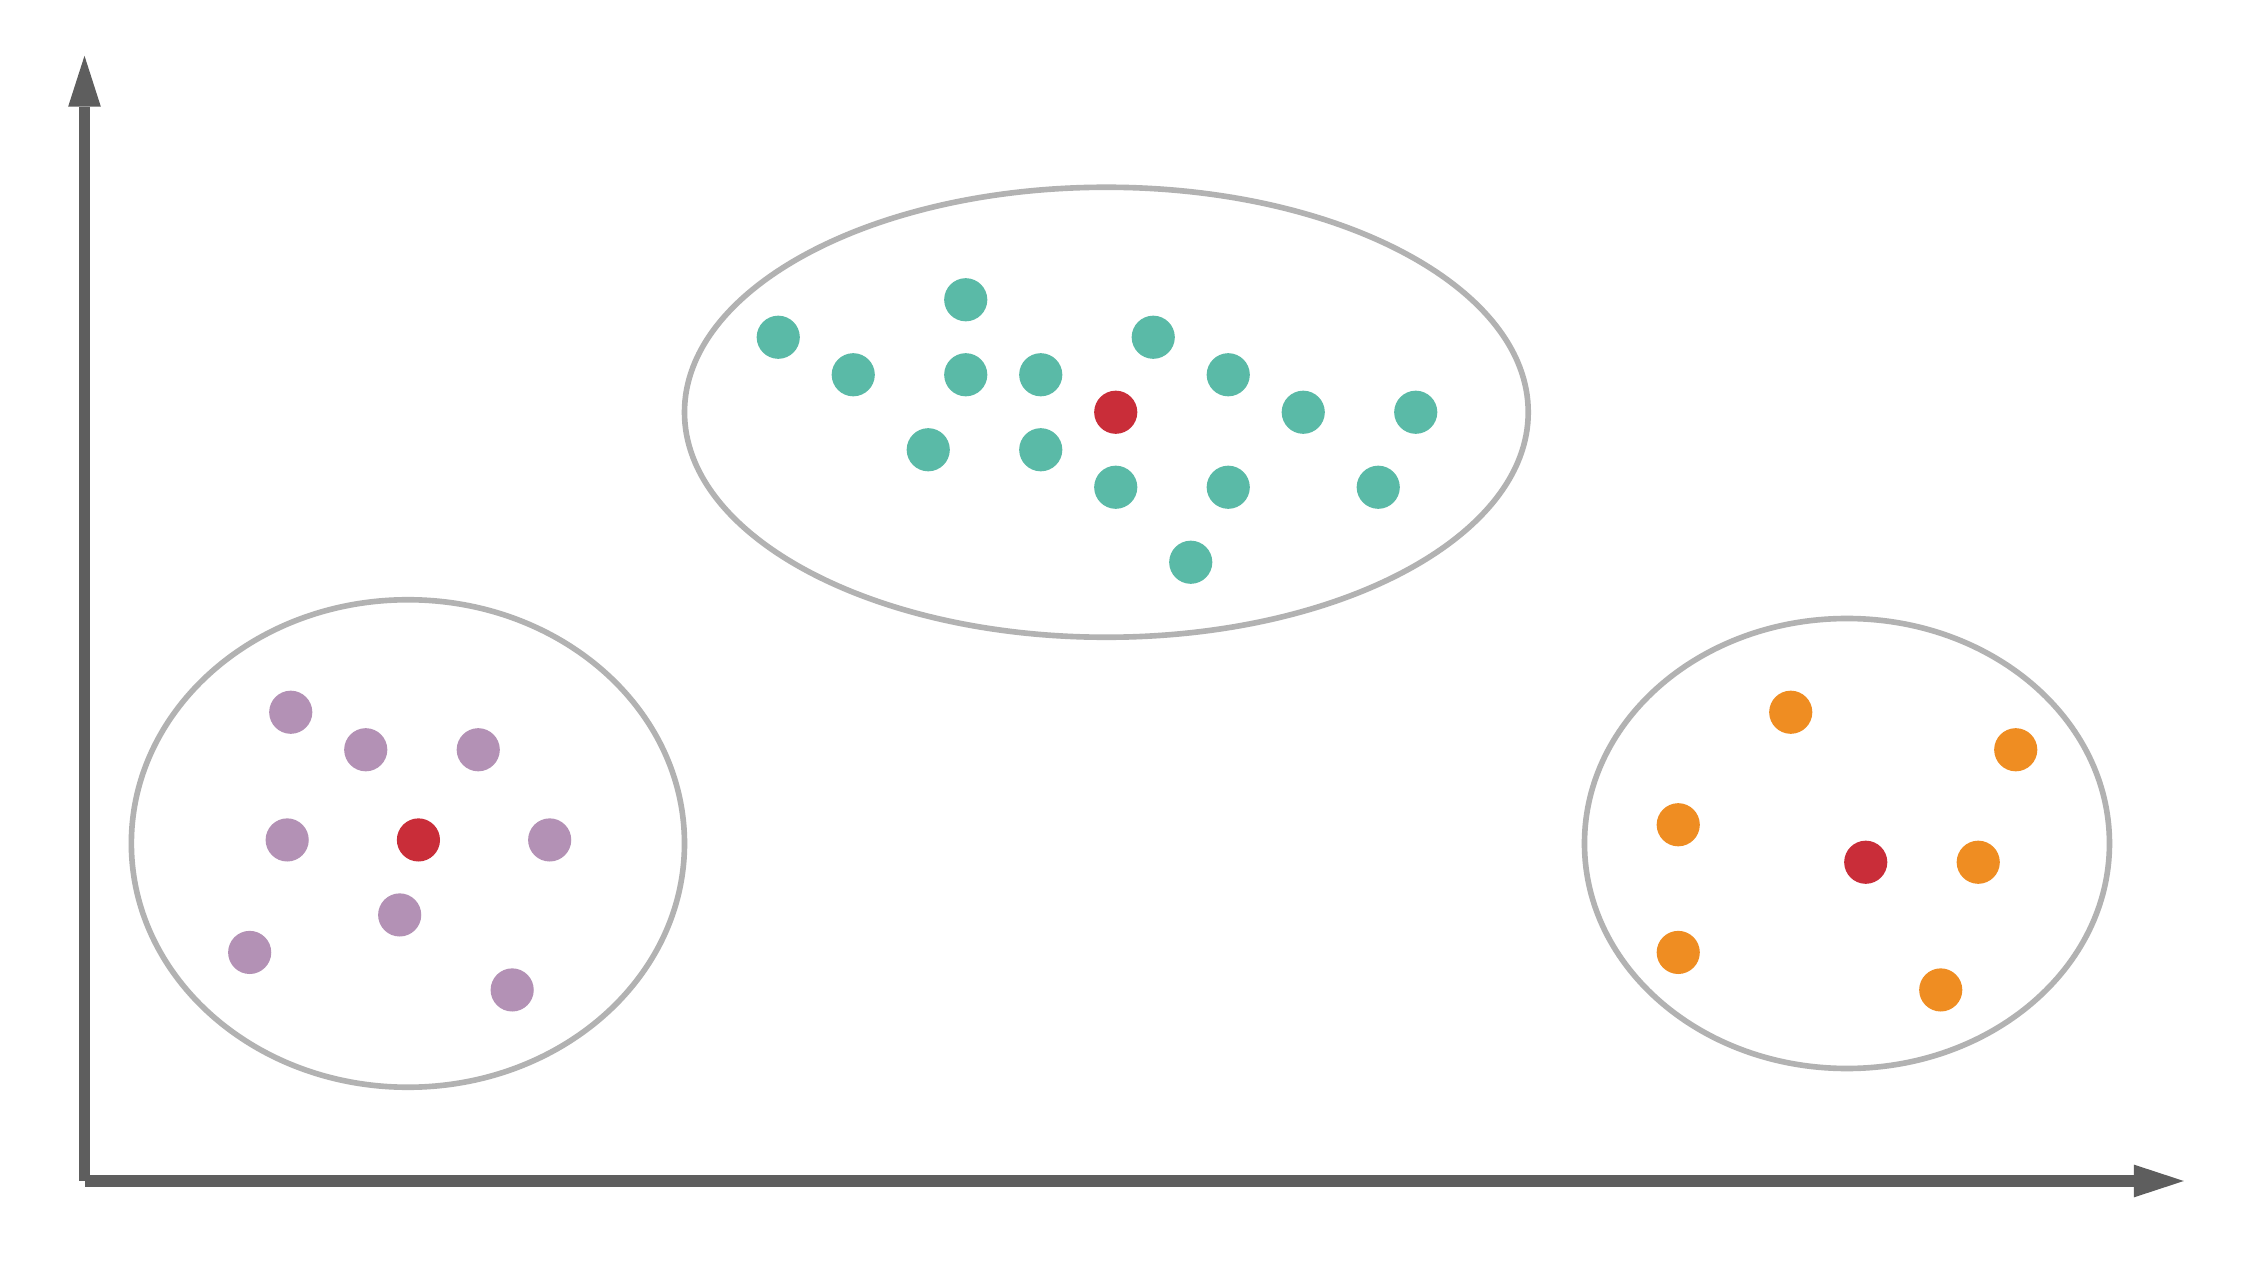
\includegraphics[width = 8 cm]{image/Chapters/Chapter2/Blank diagram (1).png}
    \caption{Clustering in 2D feature space}
    \label{clus}
\end{figure}


Once a proximity measure is chosen, the construction of a clustering criterion function makes the partition of
clusters an optimization problem, which is well defined
mathematically, and has rich applications in marketing, biomedical and geospatial fields \cite{jain1999data}. 

\subsection{Clustering Methods}

Clustering is ubiquitous, and a wealth of clustering methods has been developed to solve different problems in specific fields. However, there is no clustering method that can be universally used to solve all problems. Some problem examples can be described as follows: 

\begin{itemize}
    \item \textit{Group Discovery}: Clusters provide useful information for supporting a pre-processing step of discriminant analysis. 
    \item \textit{Pattern Recognition}: Clusters can be used for supporting template matching by determining similarities between two entities of the same type (e.g., points, curves, or shapes), finding patterns and regularities in data.
    
   % the information stored in the database with the incoming data. 
    \item \textit{Data Compression}: Clusters provide a summary of a data set by reducing the number of data points needed to represent a data set. This is achieved by using cluster centroids rather than the actual data points. 
    
   % its most representative object which can be a center of mass or an actual data point as a centroid.
    \item \textit{Outlier detection}: Clustering has been successfully applied to find outliers in data. % is another method in which many applications employ anomaly detection, such as intrusion detection, fraud detection. Anomaly detection is achieved by identifying outliers. 
    An outlier can be assigned to a data point very far from its cluster centroid or a cluster that deviates from the prominent clusters.
    \item \textit{Feature Reduction}: Clusters can be used for dimension reduction when the number of features in a data set is larger than the number of data points.
    \end{itemize}




%Even though labeled data can be analyzed using clustering techniques, but the strength of this unsupervised approach (or exploratory learning) lies in detecting similarities within an unlabelled dataset. 



% and these two words bring distances of each data point in the cluster which is closer to other data points than other data points in other clusters \cite{zumel2014practical}. 


% The Euclidean distance is the most common one, and this is what we applied in our work. It calculated the root of square differences between two pairs of data points.
% Manhattan distance which computes the absolute differences between two data points.
% Minkowski distance is ---
% Cosine distance is a common similarity metric in text analysis. It measures the smallest
% angle between two vectors \cite{zumel2014practical}.
% Mahalanobis distance---
% Categorical data usually applies Hamming distance which a number of attributes taking different values \cite{han2001data}.




Therefore, selecting a clustering method is an important step, as certain methods might be best-suited for a particular type of data sets in order to reflect the true nature of the data \cite{berkhin2006survey, han2011data}. Traditionally, clustering methods can be distinguished into five main categories described as follows: 

%The advantages and disadvantages of all these methods are listed next in \ref{methoda}.
%In progress

\begin{itemize}

    \item\textit{Partitioning methods:} In these methods data points are split into $k$ number of clusters. Each data point can only belong to one cluster, and each cluster must contain at least one data point. The algorithms usually require a distance threshold %the distance of new data points to the existing micro-clusters, and maybe it comes(happen) 
    to generate new clusters, specially those with spherical shapes.   %. These types of algorithms are 
    %finding clusters with spherical shapes. %, and the noise can influence the results. A very famous algorithm in this group is K-means.
    K-means is the most recognized clustering algorithm in this category due to its robustness in finding clusters that have not been explicitly labeled in the data.
    
    \item\textit{Hierarchical methods:} The aim is to build a tree-like nested structure from a set of data points \cite{swarndeep2016overview}. Initially each data point is considered as an individual cluster, and at each iteration, a proximity matrix is computed to merge similar clusters until one cluster or $k$ clusters are formed. These methods are widely used to analyze social network data. The BIRCH algorithm is an example of a hierarchical method where every data point is equally important for clustering purposes. Moreover, the concept of Clustering Feature (CF) is fundamental for summarizing the information that needs to be maintained about a cluster.
    
    %The clusters are described in the form of dendrogram. %It can be analyzed with the help of statistical method. 
    
    %the algorithm related to this group.
    %elmi
    \item\textit{Density-based methods:} Clusters are separated from each other by contiguous regions of low density of data points. They are highly efficient to find arbitrary shaped clusters and clusters with noise.  DBSCAN and OPTICS are well-known algorithms in this group.
    
    %continue to grow the given cluster as long as the density in the neighborhood. 
    
% exceeds certain threshold
    %elmi
    \item\textit{Grid-based methods:} %are a special category of density-based algorithms, where the regions consists of the grid cells. In particular, 
    The feature space is partitioned into a finite number of cells to form a grid structure and then find the clusters from the cells. These methods are efficient in mining large multidimensional data sets. STING is one of the highly scalable algorithms in this group with the ability to decompose a feature space into various levels of detail. 
   
    %elmi
    \item\textit{Model-based methods:} The main assumption is that the data points are generated by a model which can be adapted to what we know about the underlying distribution of the data. The model that we recover from the data then defines clusters and an assignment of data points to new clusters. A commonly used criterion for estimating the model parameters is maximum likelihood.
    
    %try to fit a model to the data, assuming that data are generated from k probability distributions (typically Gaussian).
\end{itemize}

The main advantages and disadvantages of these different clustering methods are summarized in Table \ref{methoda1}. 

\begin{table}[!ht]\scriptsize
% \centering
\caption{ Comparison of clustering methods}% \protect\cite{mousavi2015data}
\label{methoda1}  
\small
\begin{tabularx}{\linewidth}{p{3cm} p{5.5cm} p{5.5cm}}
\hline
 \multicolumn{1}{c}{\textit{\textbf{Categories}}} &
 \multicolumn{1}{c}{\textit{\textbf{Advantages}}}   &   
\multicolumn{1}{c}{\textit{\textbf{Disadvantages}}} 
\tabularnewline \hline
\vfill 
 \textbf{Partitioning Methods}    & 
 \begin{enumerate}[*,topsep=0pt,leftmargin=0.2cm]
 \item Easy to implement  
 \item Produce tighter clusters
\end{enumerate}
\tabitem
&       
\begin{itemize}[*,nosep,leftmargin=0.2cm]
    \setlength\itemsep{0em}
     %\item Require pre-defined value for number of clusters  THIS IS NOT CORRECT, SINCE AP DOES NOT REQUIRE THE NUMBER OF CLUSTERS
     \item Best suited for finding spherical shaped clusters
\end{itemize} 
\tabularnewline \hline

\vfill
\textbf{Hierarchical Methods}
& 
\begin{itemize}[*,nosep,leftmargin=0.2cm]
    \item Easy to handle any type of distance function   
\end{itemize}
 &       
\begin{itemize}[*,nosep,leftmargin=0.2cm]
  % \item High ambiguity of clustering criteria 
    \item High computational complexity
\end{itemize}
\tabularnewline \hline
\vfill
\textbf{Grid-based Methods}
& 
\begin{itemize}[*,nosep,leftmargin=0.2cm]
    \item Fast processing time 
    \item Effective with handling noisy data
\end{itemize}
&      

\begin{itemize}[*,nosep,leftmargin=0.2cm]
    %\item Higher value for convex clusters
    \item Limited to the Euclidean distance function
\end{itemize}
\tabularnewline \hline
\vfill
 \textbf{Density-Based Methods}
& 
\begin{itemize}[*,nosep,leftmargin=0.2cm]
    \item Fast to compute
    \item Easy to interpret clusters %as it gives higher value when clusters are dense
\end{itemize}
 &       
\begin{itemize}[*,nosep,leftmargin=0.2cm]
    \item Higher value for convex clusters compared with density-based clusters
\end{itemize}
\tabularnewline \hline
\vfill
 \textbf{Model-Based Methods}
& 
\begin{itemize}[*,nosep,leftmargin=0.2cm]
    \item Offer more flexibility
    %Number of clusters based on standard statistics 
    \item Effective in handling noisy data            
\end{itemize}
 &       
\begin{itemize}[*,nosep,leftmargin=0.2cm]
    \item Highly dependent on the hypothesized model
\end{itemize} 
\tabularnewline \hline
\vfill
\end{tabularx}
\end{table}


% % Please add the following required packages to your document preamble:
% % \usepackage[table,xcdraw]{xcolor}
% % If you use beamer only pass "xcolor=table" option, i.e. \documentclass[xcolor=table]{beamer}
% \begin{table}[]
% \caption{Comparison of clustering methods}
% \label{methoda1}
% \begin{tabular}{
% >{\columncolor[HTML]{FFFFFF}}l ll}
% \hline
% \multicolumn{1}{c}{\cellcolor[HTML]{FFFFFF}\textit{\textbf{Categories}}}  & \multicolumn{1}{c}{\cellcolor[HTML]{FFFFFF}\textit{\textbf{Advantages}}}                               & \multicolumn{1}{c}{\cellcolor[HTML]{FFFFFF}\textit{\textbf{Disadvantages}}}                                          \\ \hline
% \textbf{\begin{tabular}[c]{@{}l@{}}Partitioning \\ Methods\end{tabular}}  & \begin{tabular}[c]{@{}l@{}}*Easy to implement\\ *Produce tighter clusters\end{tabular}                 & \begin{tabular}[c]{@{}l@{}}*Best suited for finding spherical \\ shaped clusters\end{tabular}                        \\ \hline
% \textbf{\begin{tabular}[c]{@{}l@{}}Hierarchical \\ Methods\end{tabular}}  & \begin{tabular}[c]{@{}l@{}}*Easy to handle any type \\ of distance function\end{tabular}               & *High computational complexity                                                                                       \\ \hline
% \textbf{\begin{tabular}[c]{@{}l@{}}Grid-based\\  Methods\end{tabular}}    & \begin{tabular}[c]{@{}l@{}}*Fast processing time\\ *Effective with handling \\ noisy data\end{tabular} & \begin{tabular}[c]{@{}l@{}}*Limited to the Euclidean \\ distance function\end{tabular}                               \\ \hline
% \textbf{\begin{tabular}[c]{@{}l@{}}Density-Based\\  Methods\end{tabular}} & \begin{tabular}[c]{@{}l@{}}*Fast to compute\\ *Easy to interpret clusters\end{tabular}                 & \begin{tabular}[c]{@{}l@{}}*Higher value for convex \\ clusters compared with \\ density-based clusters\end{tabular} \\ \hline
% \textbf{\begin{tabular}[c]{@{}l@{}}Model-Based\\  Methods\end{tabular}}   & \begin{tabular}[c]{@{}l@{}}*Offer more flexibility\\ *Effective in handling noisy\\  data\end{tabular} & \begin{tabular}[c]{@{}l@{}}*Highly dependent on the\\  hypothesized model\end{tabular}                               \\ \hline
% \end{tabular}
% \end{table}





\subsection{Affinity Propagation Clustering}

% $O(N^2logN)$ where N is the number of data points. It can be imagined that if the number of data points is very huge, then it is impossible to do clustering using AP
Affinity propagation (AP) is a partitioning-based clustering algorithm that was first introduced by Frey and Dueck in 2006 \cite{frey2006mixture}. AP is based on the concept of "message passing" between data points that plays an important role in finding the best candidate data point that becomes a cluster centroid \cite{frey2007clustering, jiang2019exemplar}. 



%It means to find data points with the maximum similarity to others. The advantage of AP to compare with many clustering algorithms is that this Algorithm does not require the number of clusters as an input, and it makes it unique between many clustering algorithms.


Unlike clustering algorithms such as k-means, affinity propagation does not require the number of clusters to be determined or estimated before running the algorithm. It considers all data points as a potential centroids until an optimal set of clusters and their respective centroids are found through an iterative process. %as illustrated in Figure \ref{APPi}. 
% \todo[inline]{Please explain the contents of this figure}

%illustrates the gradually emerging of clusters and centroids, but the tenth iterations show the uncertainly of having clusters shows with the faded blue lines until the last and final iteration to find a good cluster solution. NOT POSSIBLE TO UNDERSTAND THE MESSAGE OF THIS PARAGRAPH

% \begin{figure}
% \centering
% 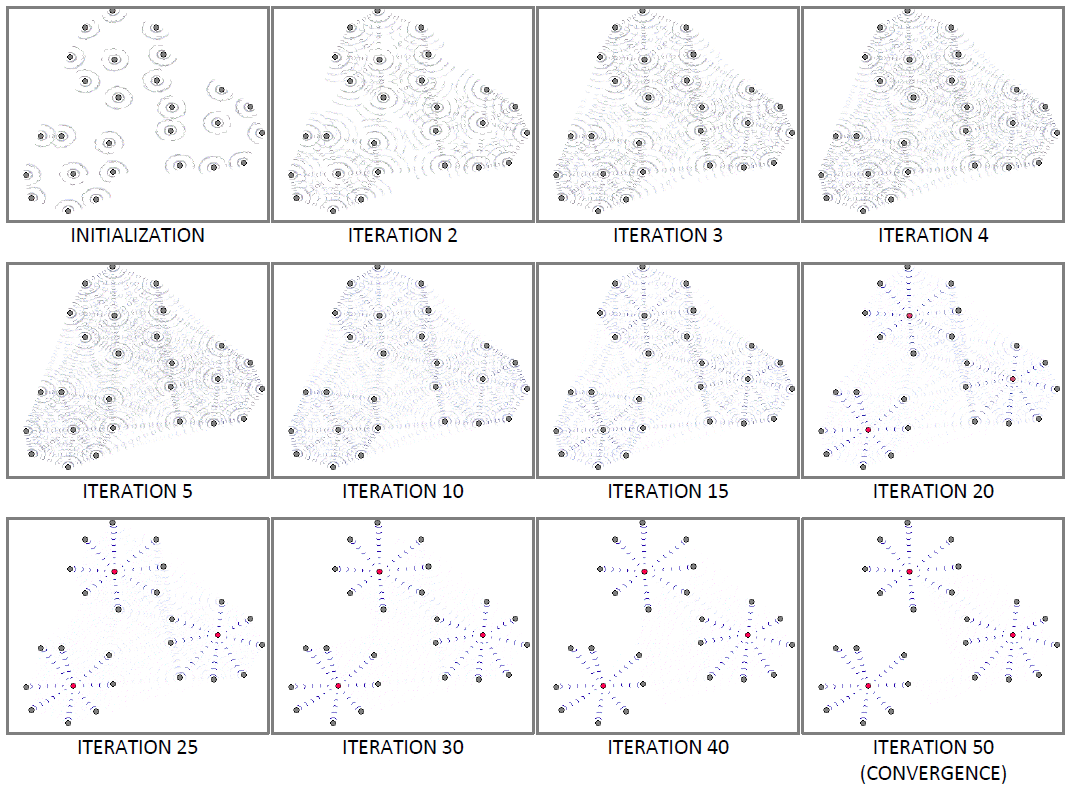
\includegraphics[width = 13 cm]{image/Chapters/Chapter2/APDurek.PNG}
% \caption{Iteration process of affinity propagation (Source: \protect\cite{dueck2009affinity})}
% \label{APPi}
% \end{figure}


The AP algorithm supports similarities that are not symmetric, and it is not dependent on initialization found in other clustering algorithms \cite{refianti2017time}. In order to apply AP for any data set two conditions should be met: no missing or null data in the inputs and the feature space should contain only numeric, not categorical data. However, it has a significant speed problem, particularly for clustering large volume of data. Affinity Propagation needs $O(N^2T)$ time to update a message where $N$ and $T$ represent the number of data points and the number of iterations \cite{frey2007clustering}. 


The AP algorithm is based on the computation of four matrices: similarity matrix, responsibility matrix, availability matrix, and criterion matrix. They can are described as follows:

\begin{itemize}

  \item\textit{Similarity Matrix:}
  Every cell value in the similarity matrix $s(i,j)$ corresponds to an element \textit{k} representing how similar/dissimilar two data points are in a feature space. This element \textit{k} is defined as the negative of the Euclidean distance between the two data points. The greater the distance between any two data points, smaller is the \textit{k} between them. The \textit{k} values of the off-diagonal cells will dictate the number of clusters formed, in such a way that the smaller the index value (value	$\leq$0), fewer number of clusters is obtained.
  %gives information about any inputs. It shows data points with is how appropriate to be the cluster-head for data point \textit{i}. 
  %Every cell has values that correspond to how similar two objects are. It is a diffident method to calculate the values for diagonal values and non-diagonal values.  The diagonal values,  Cells are filled with the lowest number among all the cells. The non-diagonal values are the negation of the sum of the squares of the differences between participants.
  \item\textit{Responsibility Matrix:} The matrix $r(i , k)$ quantifies how well-suited element $k$ is, to be a cluster centroid for element $i$, taking into account the nearest contender $k^{\prime}$ to be a cluster centroid for $i$.
  
  %Cells contain values that correspond to how responsible one data point is for another. It is better to say how responsible it is to be a part of another object or related to another object. 
  We initialize the matrix $R$ with zeros, and compute the next values using the equation:

    \begin{equation}
        r(i, k) \leftarrow s(i, k) - \max\limits_{k' s.t. k' \neq k}\{ a(i, k') + s(i, k') \}
    \end{equation}
 
 The goal is to quantify how similar is $i$ to $k$, compared to some $k^{\prime}$, taking into account the availability of $k^{\prime}$.   
    
  \item\textit{Availability matrix:} The matrix $a(i,k)$ quantifies how appropriate is it for $i$ to choose $k$ as its cluster centroid, taking into account the support from other elements that $k$ should a centroid. Availability is self-responsibility of $k$ plus the positive responsibilities of $k$ towards elements other than $i$ as shown in the following equation:
  
    \begin{equation}
        a(k, k) \leftarrow \sum\limits_{i' \neq k}\max(0, r(i', k))
    \end{equation}
  
  The matrices $R$ and $A$ matrices are iteratively updated. This procedure may be terminated after a fixed number of iterations, after changes in the values obtained fall below a threshold, or after the values stay constant for some number of iterations.
  
  
%   \begin{equation}
%         (i, k) \leftarrow \min\{0, r(k,k) + \sum\limits_{i' s.t. i' \notin \{i, k\}}{\max\{0, r(i', k)\}}
%     \end{equation} 
  
 % This matrix contains values that correspond to how available one object is to be a centroid for another object. With this means, how available one object is for a cluster to be a centroid of a cluster, and diagonal values is the sum of all positive responsibility values in the column excluding the object self-responsibility. 
 % The availability diagonal values are determined by the following formulas:

  Figure \ref{abc} illustrates how the AP algorithm sends responsibility and availability messages to data points \protect\cite{dueck2009affinity}. Responsibility $r(i,k)$ is the message from data point $i$ to candidate centroid $k$ and answer relies on determining if point $k$ is well-suited to be a centroid for data point $i$. Availability $a(i,k)$ sends a message from centroid $k$ to data point $i$ to find how well it would be for point $i$ to choose point $k$ as a centroid. 
    


    \begin{figure}
    \centering
    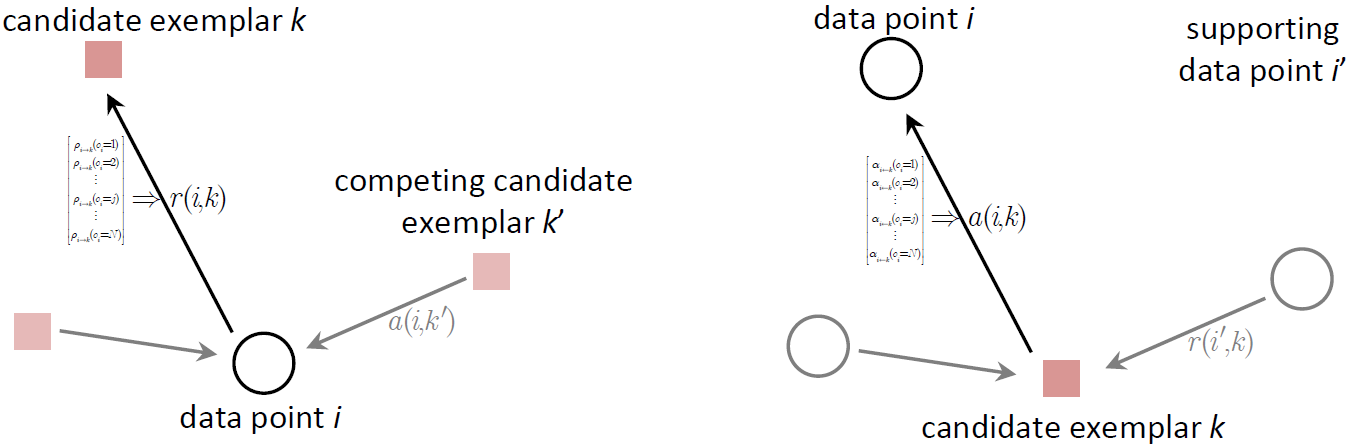
\includegraphics[width = 13 cm]{image/Chapters/Chapter2/APmessage.PNG}
    \caption{Message passing based on responsibility and availability matrices}
    %AP sends two types of message towards other data points: responsibility and availability \protect\cite{dueck2009affinity}. Responsibility $r(i,k)$, is the message from data $i$ to candidate centroid $k$ and the respond back to figure out if point $k$ is well suited as a centroid for point $i$.    Availability $a(i,k)$, send a message from centroid $k$ to point $i$ to find how well it would be for point $i$ to choose point $k$ as a centroid. ##########THIS IS TOO MUCH TEXT TO BE PART OF A FIGURE CAPTION###########}
    \label{abc}
    \end{figure}


  \item\textit{Criterion matrix:} This matrix is calculated after the iteration process is terminated.The $c (i,k)$ matrix is the sum of $R$ and $A$. An element $i$ will be assigned to an exemplar $k$ which is not only highly responsible but also highly available to $i$  as shown in 
    
    \begin{equation}
        c(i, k) \leftarrow r(i, k) + a(i, k)
    \end{equation}
    
  %\todo[inline]{put the equation for the C matrix here}
  
  %Lastly, in the criterion matrix, each cell is the sum of the availability matrix and responsibility matrix. The highest criterion values of each row are designated as a centroid.

The element with the highest criterion value in each row would be designated to be a cluster centroid. Elements that have the same centroid will be in the same cluster.







\end{itemize}

The AP clustering algorithm used in this thesis is described in Algorithm \ref{APo}. The Python code used in this work is available at https://scikit-learn.org/ open source repository. Four hyperparameters are used for tuning the clustering process using AP. They are described as follows: 

\begin{itemize}

\item Damping Factor is the extent to which the current value is maintained relative to incoming values (weighted 1 - damping). This is used to avoid numerical oscillations when updating messages.

\item Maximum number of iterations.

\item Convergence is the number of iterations with no change in the number of estimated clusters that stops the convergence.

\item Preference is the number of centroids is influenced by the input preferences value. If the preferences are not passed as arguments, they will be set to the median of the input similarities.

\item Affinity is the selection of which distance function to use.


    % \item\textit{Preference Parameter:} determines a p how likely is a data point $i$ to be chosen as a centroid. This value is in the diagonal of similarity matrix. The number of identified clusters can be increased or decreased by changing this parameter correspondingly, and a good choice is to set the preference to be the median of all the similarities between data points \cite{li2012improved}.
    % %This value for the e-counter dataset for the online phase is -4 and the value of the offline phase is -1. This number is a median value of the similarity matrix.
    % \item\textit{Damping factor:}  is the extent to which the current data point is maintained relative to incoming data points. Damping should be between 0.5 to 1. 
    % \item\textit{Maximum number of iteration:}  defines the maximum number of iterations. The default value for both online and offline phase is 100.
    % \item\textit{Convergence iteration:}  is the number of iterations with no change in the number of estimated clusters that stop the convergence.
\end{itemize}

\begin{algorithm}[]
 \caption{Affinity Propagation Algorithm}
\label{APo}
    \SetKwInOut{Input}{Input}
    \textbf{Input:} Data $d=(d_{1}, d_{2},...,d_{n})$\\
    \textbf{Hyper-parameters:}
        {Preference, Damping,  $conv_{it}$, $max_{iter}$}\\
\textbf{Output:} {Cluster centroids $C_1, ..., C_k$, branch points }\\
  	\SetKwFunction{FIROC}{AP}
    \SetKwProg{Fn}{Function}{:}
    \Fn{\FIROC{$d$}}{
        \textbf{Initialization:}\\
        {Similarity Matrix: S $\forall$ i, k:  s(i, k)} = 0\newline
        {Availability Matrix: A $\forall$ i, k:  a(i, k)} = 0\newline
        {Responsibility Matrix: R $\forall$ i, k:  r(i, k)} = 0\newline
        {Criterion Matrix: E $\forall$ i, k:  e(i, k)} = 0\newline
     \textbf{Compute S:}
        {$\forall i, k:  s(i, k) \leftarrow -\norm{V_i - V_k}^2 where V_i = (M_i, S_i) $}\newline
  	 \emph{
  	 \While{$r(i,k)\ \&\ a(i,k) \neq $convergence}{
  	 \textbf{Compute R:}\newline
  	       $r(i, k) \leftarrow s(i, k) - \max\limits_{k' s.t. k' \neq k}\{ a(i, k') + s(i, k')$ \}\newline
  	       \textbf{Compute A:}\newline
  	       $a(i, k) \leftarrow \min\{0, r(k,k) + \sum\limits_{i' s.t. i' \notin \{i, k\}}{\max\{0, r(i',k) \}}$\newline
  	       \textbf{no-diagonal A:}\newline
  	       $a(i, k) \leftarrow \sum\limits_{i' \neq k}\max(0, r(i', k))$\\
  	       \textbf{cluster assignment: $E = (E_1,..E_n)$ $E = argmax[a(i,k) + r(i,k)]$}
  	       }
  	       }
  	       
          	  }  \textbf{Results }C = $(C_1, ..., C_k)$

\end{algorithm}





%To improve the algorithm performance, hyper-parameters should be considered. These parameters are variables that control the performance and structure of any machine learning model and they are grouped in four, Preference, damping maximum iteration, and convergence iteration. These parameters are described below.

%elmi-In un-convergent cases, we have to increase lam manually and gradually and rerun AP until the algorithm converges. Another choice is to use a big damping factor close to 1 to eliminate oscillations, but AP will run very slow. Both choices may consume plenty of time, especially for a large data set
%    \item Number of initial data points: 500 items from the head of the stream
 %   \item Threshold($\epsilon$): This number is the average distance between data points and exemplars in the first phase. For e-counter dataset it is equal to 1.

%) preferences for each data point that is more likely to be chosen as an exemplar. 2) $convergence\_iter$ is the number of iterations with no change in the number of estimated clusters that stop the convergence. 3) damping factor (between 0.5 and 1) is the extent to which the current data point is maintained relative to incoming data points (weighted 1 = damping); and 4) $max\_iter$ defines the maximum number of iterations.







% \subsection{K-means Clustering} \label{kmeansalgo}
% \todo[inline]{Nasrin you need to improve this section}

% K-means was first introduced by J.MacQueen in 1967 \citet{macqueen} as a method for partitioning numerical data into isotropic clusters.% and is not as versatile as single link algorithms. 
% It is a distance based algorithm  which aims to assign each observation to a cluster with the nearest mean (cluster centroid) based on it's distance from the centroid. The number of clusters need to be defined in advance. This is not straightforward task since no prior information is generally available.

% K-means is a suitable algorithm due to its simplicity and low computational costs. The complexity for $n$ iterations of the K-means algorithm is $O(n*K*m*N)$, where $n$ is a number of iterations, $K$ set of macro clusters, $m$ is the sample size with N attributes.  This linear complexity is one reason for the popularity of the Kmeans algorithms. It guarantees convergence and scales quite well to large datasets owing to lower memory requirements. The algorithm can be generalized to clusters of different shapes and sizes, such as elliptical clusters. Other reasons which make the algorithm so popular are a straightforward interpretation of clusters, simplicity of implementation, fast convergence, and adaptability to sparse and large data \cite{dhillon2001concept}.

% However, this algorithm is receptive to noisy data or outliers (one data point as an outlier can increase the squared error dramatically). It is suitable for data with spherical/convex clusters and well defined mean values. The output of K-Means algorithm depends on the initial value of the centroids which are the basis for the cluster determination. In essence, it is an optimization problem where a local optimal clustering can be achieved, whereas a global optimal is not always guaranteed. It is advised to run the algorithm multiple times in order to reduce the chances of a local minima solution. %It is a heuristic algorithm in which the final clustering results highly depend on the initial settings, although a reasonably good approximation is possible. 

% The main goal of K-means as a partitioning algorithm is to minimize the sum of the distances between the n data points and their representative cluster centroids into k sets $(S = s_1,...,s_n)$ and cluster them in an iterative manner. In the other words, its objective is to find:

% \begin{equation}
%     \sum_{i=1}^k \sum_{x \in S_i} \norm{x-\mu}^2
% \end{equation}

% Where $\mu$ is the mean of data points in $S_i$. However, the pre-assumption in the above equation is that the distance between the data points is the squared Euclidean distance and computed as $\norm{x - \mu}^2$. Although there are other distance metrics to find the closest distance, the Euclidean distance is widely used by other researchers owing to it's easy interpretation with low dimensional data. 

% The K-means algorithm consists of the following steps that are illustrated in Figure \ref{ite}.
% \begin{enumerate}
%     \item Randomly select k points as centroids of clusters based on the predefined value of k. These data points describe the initial set of centroids.
%     \item To create the k clusters, every data point from the dataset is assigned to the nearest centroid. The Euclidean distance is used for calculating the distance between each data point and the initial centroids. 
    
%     \item After all the data points have been assigned to their closest groups, the positions of the k centroids is recalculated by averaging all of the data points assigned in each cluster.
    
%     \item  Steps 2 and 3 are repeated until convergence is reached. This is achieved if the centroid values do not change further, the sum of distances between the data points and the centroid of each cluster does not change, the data points assigned to all clusters are the same as the previous assignment, or the maximum iteration number has been reached in case the algorithm is given a fixed iteration.
% \end{enumerate}

% \begin{figure}
% \centering
% 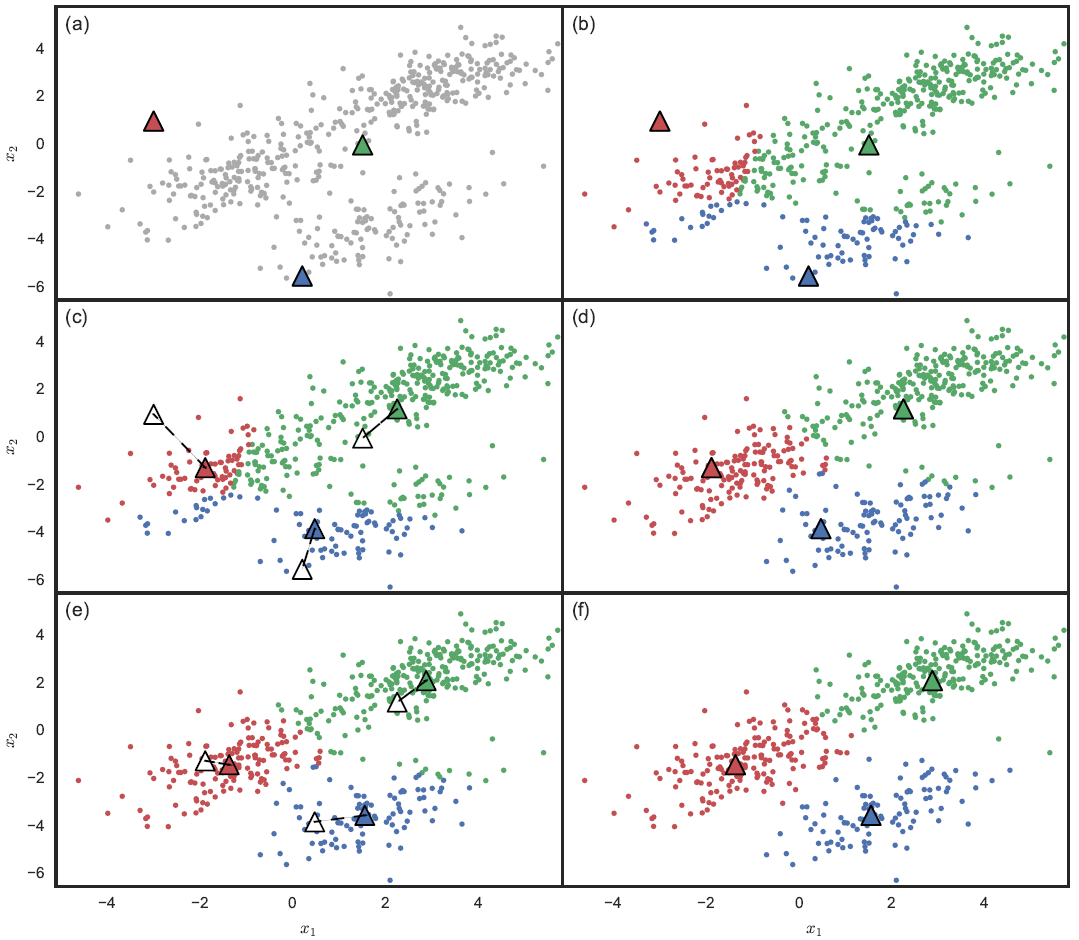
\includegraphics[width = 10 cm]{image/Chapters/Chapter2/kmeanshif.png}
% \caption{K-means Algorithm: finding clusters in a 2D data space iteratively \protect\cite{benavente2017automatic}. (a)cluster centroids initialized randomly, (b) data points map to the closest centroids, (c) centroids are moved to the mean of each cluster map points, (d,e,f) steps b and c are repeated iteratively until convergence.}
% \label{ite}
% \end{figure}

% % In the next step,  the centroids are moved to the mean of each cluster's mapped points which ${\mu_k}$ is the mean of cluster $k$ :
% % \begin{equation}
% %     {\mu_k} = \frac{1}{{N_k}}\sum_{q=1}^{{N_k}} {x_q}
% % \end{equation}

% %In this formula, $N_k$ is the number of instances belonging to cluster $k$
% % Finally, these process will be repeated until convergence. 


% % The K-means algorithm starts with the K initial set of cluster-centers and iteratively updates it to decrease the error function. A proof of the finite convergence of the K-means type algorithms is given in \cite{selim1984k}. 

% The K-means clustering algorithm that has been used in this thesis is described in Algorithm \ref{kmeanalgo}. The Python code for this algorithm as well as AP is available at https://scikit-learn.org/ open source repository. 



% \begin{algorithm}[H]
% \SetAlgoLined
% \small
% \textbf{Input:} {Data: $X$ = ${x_1,..., x_n}$}\\
% \textbf{Hyper-parameters:} {Number of clusters k, $max\_iter$}\\
% \textbf{Output:} {Set of cluster with the centroids $C = {c_1,..., c_k}$ }\\
% \textbf{Initialization:} {Set $\mu_i$, $i = 1,..., k$ to random data points }\\
% \While{(Convergence)}{
%   \For{i= 1 : n}{
%     \small\color{blue}\texttt{Assign each data point to the closest centroid:}
%     \color{black}\\
%     R_{ij} =  \arg \min_j ||x_i - \mu_j||^2, 
%     j \in 1, ..., k 
  
%   }
  
%   \For{j = 1 : k}
%   {
%     \small\color{blue}\texttt{Update each centroid by the mean value of data points within each cluster:}
%     \color{black}\\
%     n_j = \sum_{i=1}^n R_{ij}\\
%     \mu_j = \frac{1}{n_j} \sum_{i = 1}^n R_{ij} x_i
    
%   }
%  }
% {

% \textbf{return} {$\mu_1 , ... , \mu_k$\\ }
% }
%  \caption{ K-means Clustering Algorithm}
%  \label{kmeanalgo}
% \end{algorithm}

%  % \begin{equation}
% % J = \sum_{n=1}^{N} \sum_{k=1}^{K} r_{nk} ||x_n - \mu_k||^2
% % \label{eqn:kmeans_objective_function}
% % \end{equation}
 
 
 
% % Figure \ref{kmAlgo} presents the pseudo-code of K-means algorithm.

% % \begin{figure}
% % \centering
% % 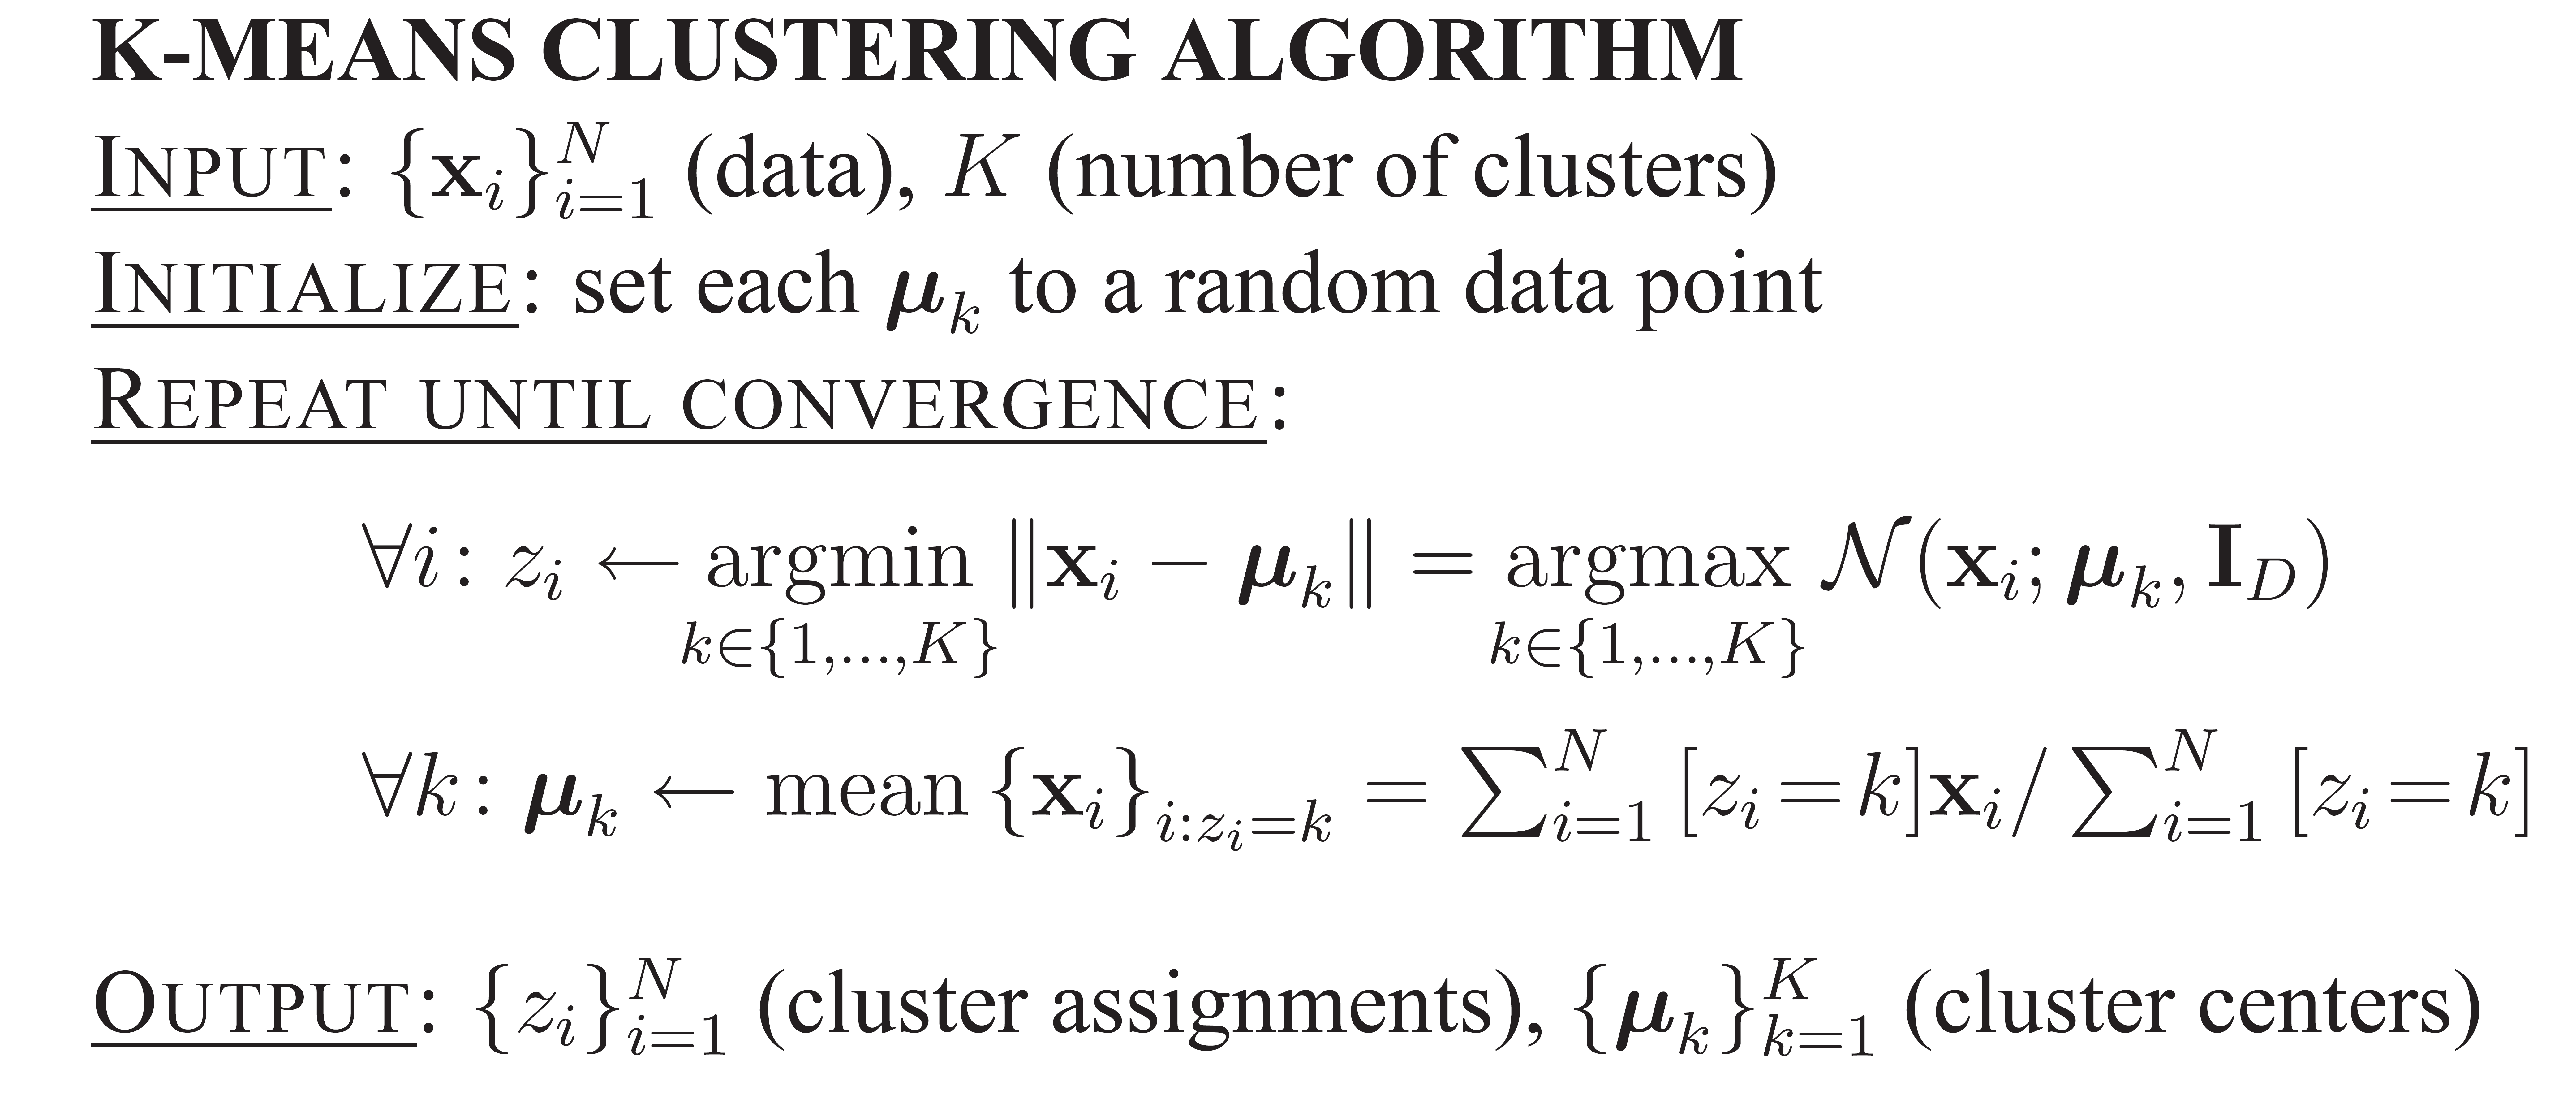
\includegraphics[width = 10cm,height = 4cm]{image/Chapters/Chapter2/6.png}
% % \caption{K-means pseudocode }
% % \label{kmAlgo}
% % \end{figure}
% \todo[inline]{make a proper for the algorithm}

% %%Elmi
% % The similarity measure on numeric attributes is the square Euclidean distance; the similarity measure on the categorical attributes is the number of mismatches between objects and the cluster prototypes.

%  %%%%%%%%%%%%%%%%%%%%%%%%%  ELMI

% % A number of convergence conditions are possible. For example, the search
% % may stop when the partitioning error is not reduced by the relocation of the centers.
% % This indicates that the present partition is locally optimal. Other stopping
% % criteria can be used also such as exceeding a pre-defined number of iterations.


% % The Achilles heel of the K-means algorithm involves the selection of the initial partition. The algorithm is very sensitive to this selection, which may make the difference between global and local minimum.
% % K-Means is one of the simplest unsupervised learning algorithms that solve the well known clustering problem. The procedure follows a simple and easy way to classify a given data set through a certain number of clusters (assume k clusters) fixed a priori.The main idea is to define k centroids, one for each cluster. These centroids should be placed in a cunning way because of different location causes different result. So, the better choice is to place them as much as possible far away from each other.The next step is to take each point belonging to a given data set and associate it to the nearest centroid. When no point is pending, the first step is completed and an early group is done. At this point, it is needed to re-calculate k new centroids as centers of the clusters resulting from the previous step. After these k new centroids, a new binding has to be done between the same data points and the nearest new centroid. A loop has been generated. As a result of this loop it may notice that the k centroids change their location step by step until no more changes are done. In other words centroids do not move any more.Finally, this algorithm aims at minimizing an objective function, in this case a squared error function. The objective function

% % \begin{equation}
% %     W(s,c) = \sum {k=1}^K\sum{iE S_k} \norm{y_i - c_k}^2
% % \end{equation}
% % Where S is a K-cluster partition of the entity set represented by vectors yi (iI) in the M-dimensional feature space,consisting of non-empty non-overlapping clusters Sk, each with a centroid ck (k=1,2,…K).
% % ###############













% %%%%%%%%%%%%%%%%%%%%%%%%%%%%%%%%%%%%%%%%%%%%%%%%%


% There are several approaches for determining the number of clusters for K-means clustering algorithm such as elbow method, Silhouette score, information criterion approach or cross-validation \cite{kodinariya2013review}.



% \noindent\textbf{Elbow Method:}

% Elbow method is a technique used for K-means algorithm to find the optimal number of clusters by fitting the model with the range of value for $k$ clusters. In this method if the line chart is assumed as an arm, then the elbow or the point of inflection on the curve as shown in Figure \ref{elb} is the best fit for the model. The scoring parameter can be distortion, Silhouette, and Caliński or many other parameters. Distortion computes the average of squared distance from each point to its assign centroid. This distance is usually is a Euclidean distance. Silhouette calculates the mean of Silhouette coefficient of all data points. Caliński score computes the ratio of dispersion between and within clusters.



% \begin{figure}
% \centering
% 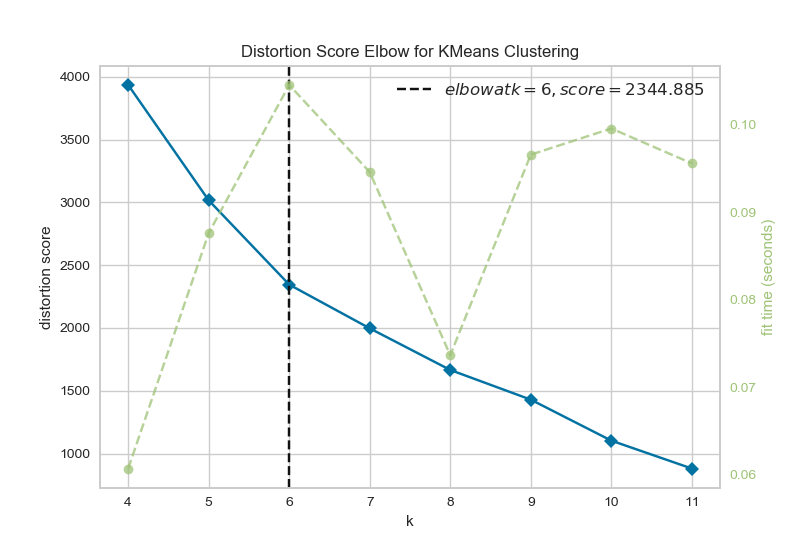
\includegraphics[width = 0.8\textwidth]{image/elbow.png}
% \caption{The elbow curve found for a $k$ range from 4 to 11 clusters. The black dotted line is optimal the number of clusters determined by the elbow method}
% \label{elb}
% \end{figure}

% The elbow method is suitable for small $k$ values. As the $k$ value increases, the average distortion degree becomes smaller. The number of data points in each category decreases, and they are closer to the center of gravity. As the $k$ value increases, the position where the improvement effect of the distortion degree decreases the most is the k value corresponding to the elbow  


\section{Streaming Cluster Analysis }
% \todo[inline]{SEQUENCE FOR THIS SECTION IS ONLINE/OFFLINE +  TIME WINDOWS +ALGORITHMS}

% \todo[inline]{start thi ssection explaining why streaming clustering is important}

\subsection{Overview}

In almost all clustering methods described in the previous section, the number of data points is considered fixed, and each data point is used multiple times for computing proximity measures and matrices in order to be assigned to a particular cluster. These methods are computationally high and require large data storage.

However, with the advent of Internet of Things, and in particular indoor localization systems, a wide range of sensor technologies (e.g., e-counters, environmental, and motion sensors) and networking communication technologies (e.g., infrared, RFID, sensors, WiFi, and Bluetooth) are being used for sensing and transporting large volume of data. The data is harvested as data streams that are a sequence of digitally encoded coherent signals (packets of data or data packets). These data packets arrive according to different data rates (i.e. bandwidth), which are often expressed in bytes per second (B/s).

From a clustering perspective, a data stream $S$ is sequence of infinitive, ordered, and fast-changing stream data points $d_1, d_2, ..., d_3 $ $\xrightarrow S = {d_i}$ \cite{han2011data}. Therefore, clustering methods need to form clusters from a continuous flow of stream data points. The traditional set-up where an entire static data set is available for clustering can not be applied to data streams which continuously arrive at a rapid rate. The main issues can be summarized as follows \cite{toshniwal2013clustering}:

\begin{itemize}
    \item Previous data used in clustering analysis is static, but data streams are unbounded and non-stationary data.
    \item Streaming cluster analysis requires a process capable of partitioning the data streams continuously while taking into account restrictions of memory and time. Traditional clustering methods partition an entire data set at once, and memory requirements do not change over time. 
    %T \item Traditional clustering datasets can be accumulated in memory, but because of the enormous size of streaming data, it is impossible to store them in memory.. NOT SURE ABOUT THIS STATEMENT, BECAUSE WE HAVE MEMORY CONSTRAINTS WITH TRADITIONAL AS WELL AS STREAMING...
    \item Traditional clusters are found from accumulated data points, but streaming clusters evolve over time depending on the time window model being used to accumulate the data points.
\end{itemize}

It is important to select a time-interval for a time window model based on the trade-off between the data rate and latency, as that plays an important role in controlling which data points in the stream are going to be processed at the current time. Four main types of time window models have been proposed in the literature \cite{nguyen2015survey, mansalis2018evaluation}. They can be described as follows:

\begin{itemize}

    \item\textit{Damped Time window:} It is also referred to as time-fading model. Each data point has a different weight based on its arrival time so new data points have a higher weight than the old ones. This time window model reduces the impact of old data. It is mostly applied using density-based clustering methods. The function $f(\delta t)$ = $\mu_{\delta t}$ (0 < $\mu$ < 1) is usually used for this model where $\delta t$ is the age of a data point which is equal to time differentiation between current time and arrival time. A fading parameter $\mu$ is in the range between 0 to 1. 
    
    
    \item\textit{Landmark Time Window:} It is also known as the hopping model, is used when clustering starts from a starting point call landmark to the current time. When a new window comes, all data points from the previous landmark time window are removed. All data points are equally important.

    \item\textit{Sliding Time Window: } The most important data points are the most recent ones and old data points will be removed. The structure of the sliding time window is based on the FIFO (First-In-First-Out) principle, which a data point from the current time is used for clustering until a specific time is passed. The window has a size of $w$ in the current time $t$, will slide (s, sliding(w)) where s[t-w+1, t].
    The window size can be set based on resources, and computational process \cite{silva2013data}. This model is efficient when most recent data points are relevant for the cluster analysis.  
    
    \item\textit{Pyramidal Time Window: } It is also known as tilted time window and focuses on recent data points without discarding old data points. It applies various time granularity levels based on how recent a data point is \cite{aggarwal2003framework, nguyen2015survey}. It stores almost all data points belonging to a specific time window, and after computes a balance between storage requirements and accuracy. The old data tuples are aggregated. %, and a generic representation is enough.
    
\end{itemize}    

Figure   \ref{time1} illustrates how these time window models have been conceptualized. Time window models also handle concept-drift by changing the trends and data distribution in clustering, avoiding forming less accurate clusters as time passes. Finding patterns without storing all the stream data points is one of the main tasks of streaming cluster analysis.

%or data distribution over the time. It means This method aims to ignore outdated and historical data because they can change the trends or the data distribution.

\begin{figure}[!ht]
\centering
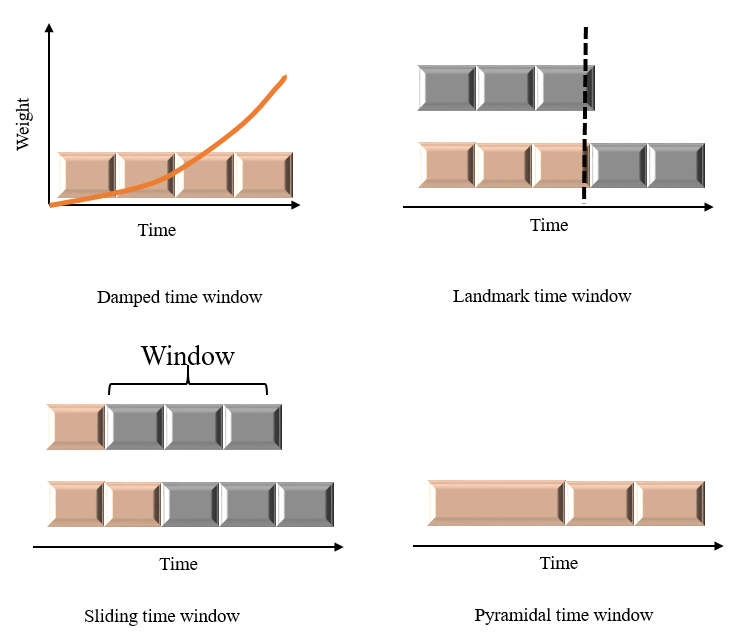
\includegraphics[width = 9cm,height = 7cm]{image/timeW.PNG}
\caption{Current time window models used with stream data points \protect\cite{carnein2019optimizing}.}
\label{time1}
\end{figure}


%Due to data stream volume, it is impossible to store entire objects. To control which part of data is going to be processed, time window models have been proposed. The other reason to use the time window model is to handle the concept-drift or data distribution over the time. It means This method aims to ignore outdated and historical data because they can change the trends or the data distribution.
%localization many applications and systems generate observations continuously, such as sensors, smart grids, network data, medical, finance, and so on. 
%indoor localization systems are described due to the potential wide range of services they can provide by leveraging Internet of Things (IoT) and ubiquitous connectivity.

%In order to keep changes for new data points and the possible shift in cluster structures, classical clustering algorithms need to be run periodically.  One major approach is to update existing clusters and merge new data points into the existing clusters by identifying emerging structures and removing outdated structures incrementally \cite{carnein2019optimizing}. This is the aim of data stream clustering algorithms in which data points come continuously in order, and the stream is possibly unbounded. Finding the pattern without storing all the observations is the main task of stream clustering.

% Data stream clustering finds clusters based on the flow of data points into the model, and it is different from traditional clustering \cite{toshniwal2013clustering}:
% \begin{itemize}
%     \item Traditional clustering data are static, the data stream is dynamic.
%     \item Traditional clustering datasets can be accumulated in memory, but because of the enormous size of streaming data, it is impossible to store them in memory.
%     \item traditional clustering results are fixed, but The data stream clustering results vary over time.
% \end{itemize}



%The methods that discuss the problem of data stream clustering can be categorized into: (1) one-pass methods that assume a unique underlying model of streaming data and cannotmstudy the evolution of data distribution, (2) evolving clustering methods that take into account the behavior of data as it may evolve over time.

%Many algorithms use similarity thresholds to decide whether an observation fits into an existing cluster or splitting the data space into a grid cells and store the location of dense or include fitting a model to represent the observed data.










% %%%%%%%%%%%%%%%%%%%%%%%%%%%%%%%%%%%%%

% Single-pass
% It is an array of the prototypes derived
% from k-median clustering. Because the first algorithms which
% were proposed simply view the stream clustering as a
% single-pass problem, the goal of these algorithms is to handle
% the infinite size of streams summarizing the stream history
% by dividing the stream into batches of predefined size m, in
% which each batch returns the k-representatives in the array.
% When the size of the representative array reaches the maximum
% boundary m these algorithms perform clustering in
% these k-representatives making the next level of representatives.


% single-pass means that you are supposed to process every element just once (and not copy it). Such algorithms obviously must be in linear time, which makes them good candidates for big data and MapReduce (if they can be somewhat divided, this is not necessarily trivial).

% Single-pass doesn't necessarily mean the results will be updateable and thus usable for online or streaming operation. However they often are, as they never need to access "old" data, and the summaries they are allowed to keep usually can be kept and updated.

% Single-pass are mostly interesting when you have too much data to keep or process more than once. So for "real time" applications and such. Obviously, the results will usually be worse than when you had full data available anytime


% %%%%%%%%%%%%%%%%%%%%%%%%%%%%%%%%%%%%%%%%%

%\subsection{Data Stream Processing}
Processing of data points using time window models can take two opposites views of the streaming problem as pointed out by Mansalis et al. (2018). The first view is to use a two-phase scheme which consists of an online component that processes stream data points and produces summary data  (e.g., micro-clusters, core-micro-clusters, temporal CF, grids, and coreset tree); and an offline component that uses the aggregated summary data to form the final clusters. In the literature of data stream clustering methods, a large number of algorithms use a two-phase scheme as shown in Figure \ref{2phase} . 

\begin{figure}[t]
\centering
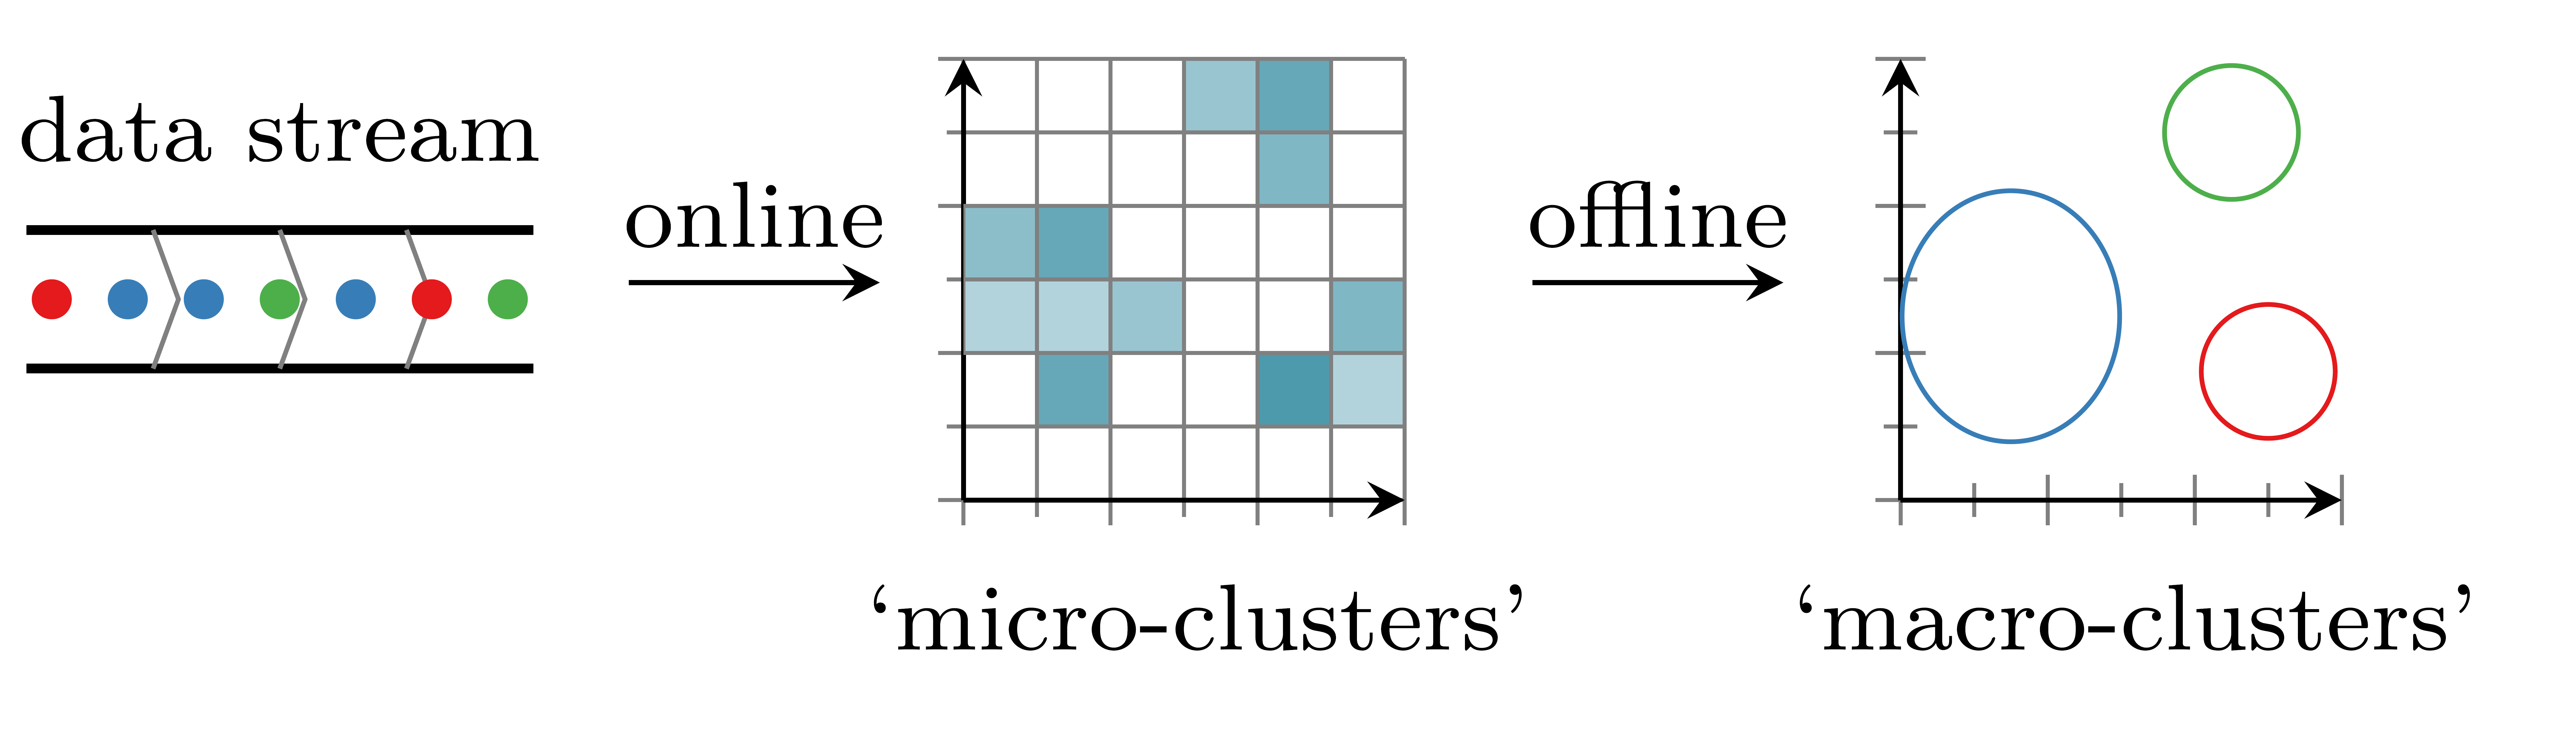
\includegraphics[width = 15cm,height = 4cm]{image/Chapters/Chapter2/2phase.png}
\caption{Overview of the two-phase processing strategy \protect\cite{carnein2019optimizing}}
%\cite{carnein2017empirical}
\label{2phase}
\end{figure}

An alternative view is to generate final clusters without the need of an offline phase. A single-pass model is maintained over a stream, and clusters are updated as new data points arrive from the stream. One of the main disadvantages of this strategy is that the evolution of the clusters can not be analyzed at different time intervals, only a final snapshot is produced.     

In this thesis, the online/offline strategy was adopted, and final clusters have been named as macro-clusters, meanwhile the the centroids of micro-clusters were used as summary data. The online component requires a process for saving the summary data in a fast manner, and is not requested to support real-time processing, but rather a very low response delay.The offline phase uses the aggregated summary data to compute the macro-clusters. It is not time-related and can happen any time by user request.




% \begin{enumerate}
%     \item\textit{Online Clustering:}These methods observe the stream clustering problem as a single-pass clustering challenge and adopt a general adaptive strategy to maintain the clusters. This model is maintained over the stream and it is updated as new data points come from the stream. Such an approach though does not allow for investigation of the cluster structure at different time intervals.
    
    % \item\textbf{Two-phase Clustering Algorithms:} All these approaches capture the location of dense in the data space and consider them as clusters. These clusters can be merged when they become similar over time. However, it is not possible to split clusters again since the underlying data was discarded and only the center of the dense region was remained \cite{aggarwal2007data}. To avoid this issue, many clustering algorithm models are divided into two parts: online and offline phases \cite{aggarwal2003framework}. Aggarwal introduced the CluStream algorithm, combined online summarization at the first stage with the offline stage using k-means. The two-phase clustering methods are visualized in figure \ref{2phase} by the grid structure.

% \begin{figure}
% \centering
% 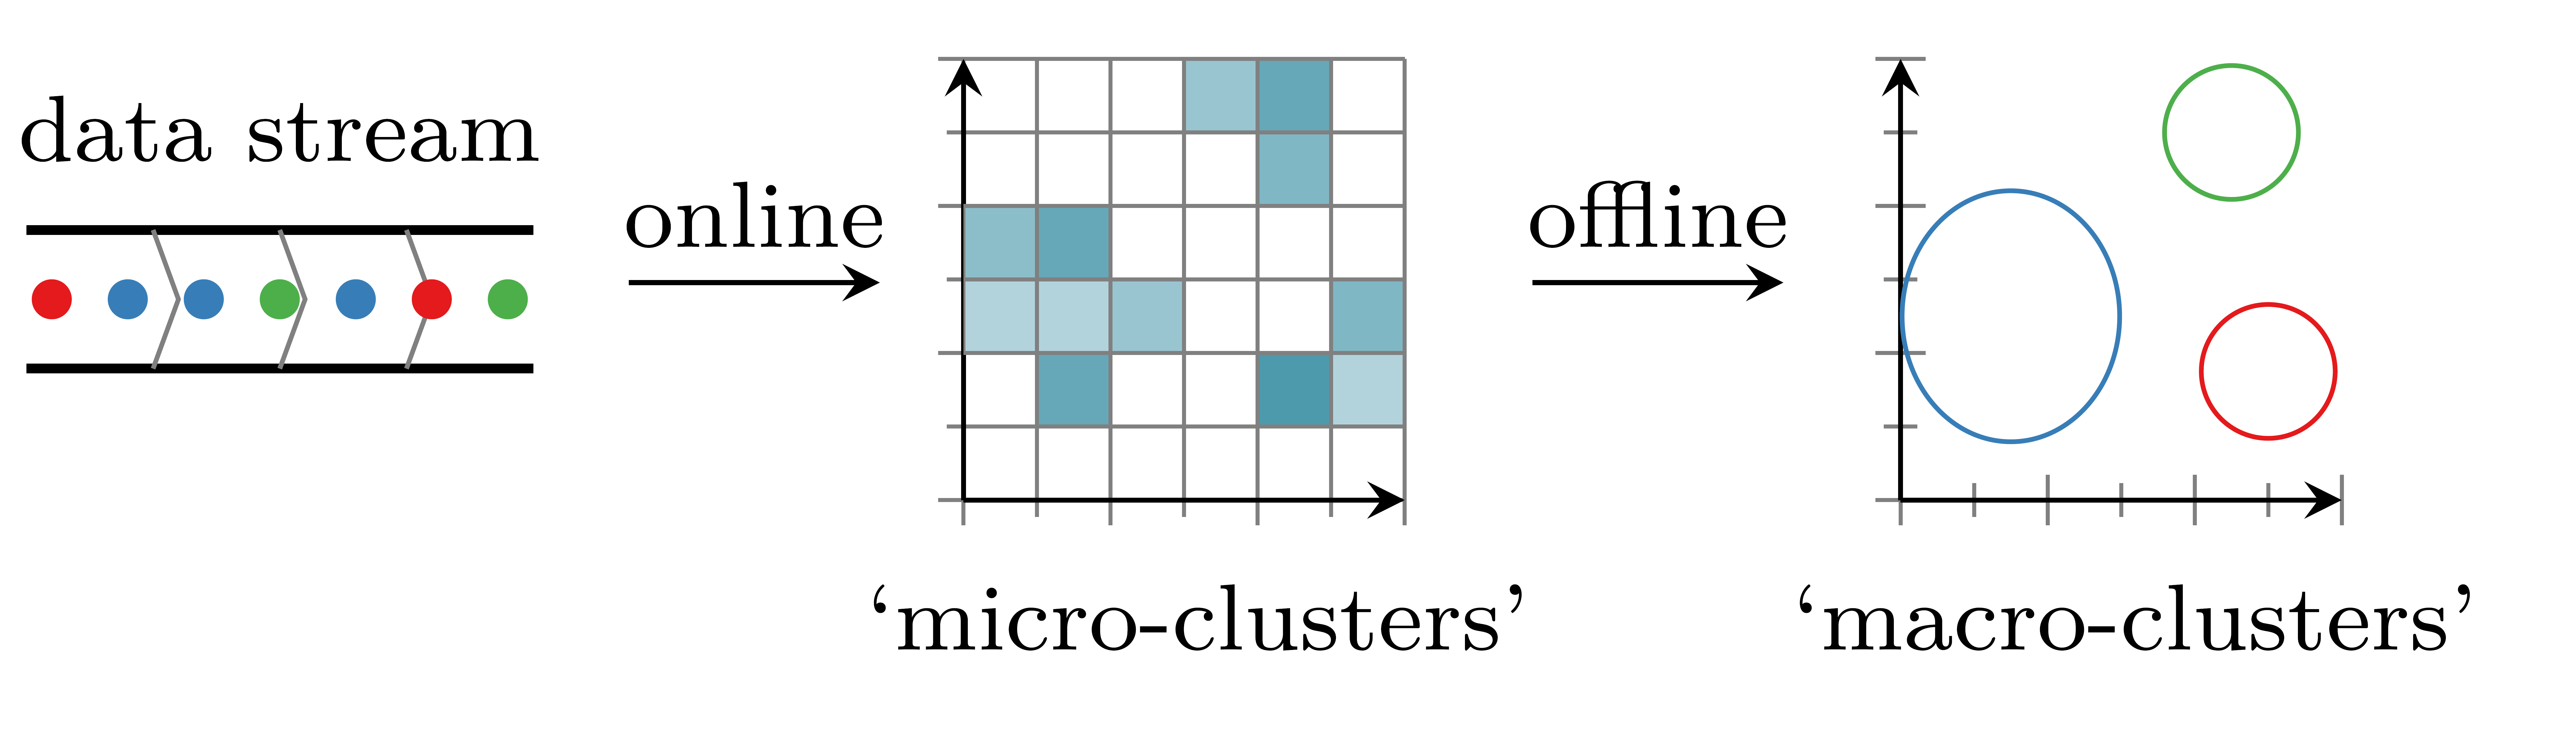
\includegraphics[width = 15cm,height = 4cm]{image/Chapters/Chapter2/2phase.png}
% \caption{Simple overview of two-phase data stream clustering algorithms \protect\cite{carnein2019optimizing}.}
% %\cite{carnein2017empirical} }
% \label{2phase}
% \end{figure}






%The second phase is triggered at the end of a designated time interval. All the centroids of clusters which have been computed by using a sliding time window model, are re-clustered to create new macro clusters and centroids. The k-means algorithm is once again employed to compute the final $k_m$ macro clusters. The advantage of applying the macro-clustering is to gain further insight from the entirety of centroids after the designated streaming window. The optimal number of $k_m$ macro clusters can be calculated by using the same method as in micro cluster which is the elbow method. The elbow method calculation can be automated or estimated at the start of micro-clustering phase. This method works by applying the k-means algorithm on micro clusters computed for all sliding time windows. 


%\subsection{Time Window Models}
\hspace{1 cm}

\subsection{Stream Clustering Methods}

Data stream clustering methods can be categorized into five leading groups according to the nature of their underlying clustering methods as previously described in Section 2.1.2. Figure \ref{method} provides an overview of the main methods developed within these categories. Table \ref{landmarkwin} provides a comprehensive overview of the data stream clustering methods. 


\begin{figure}[t]
\centering
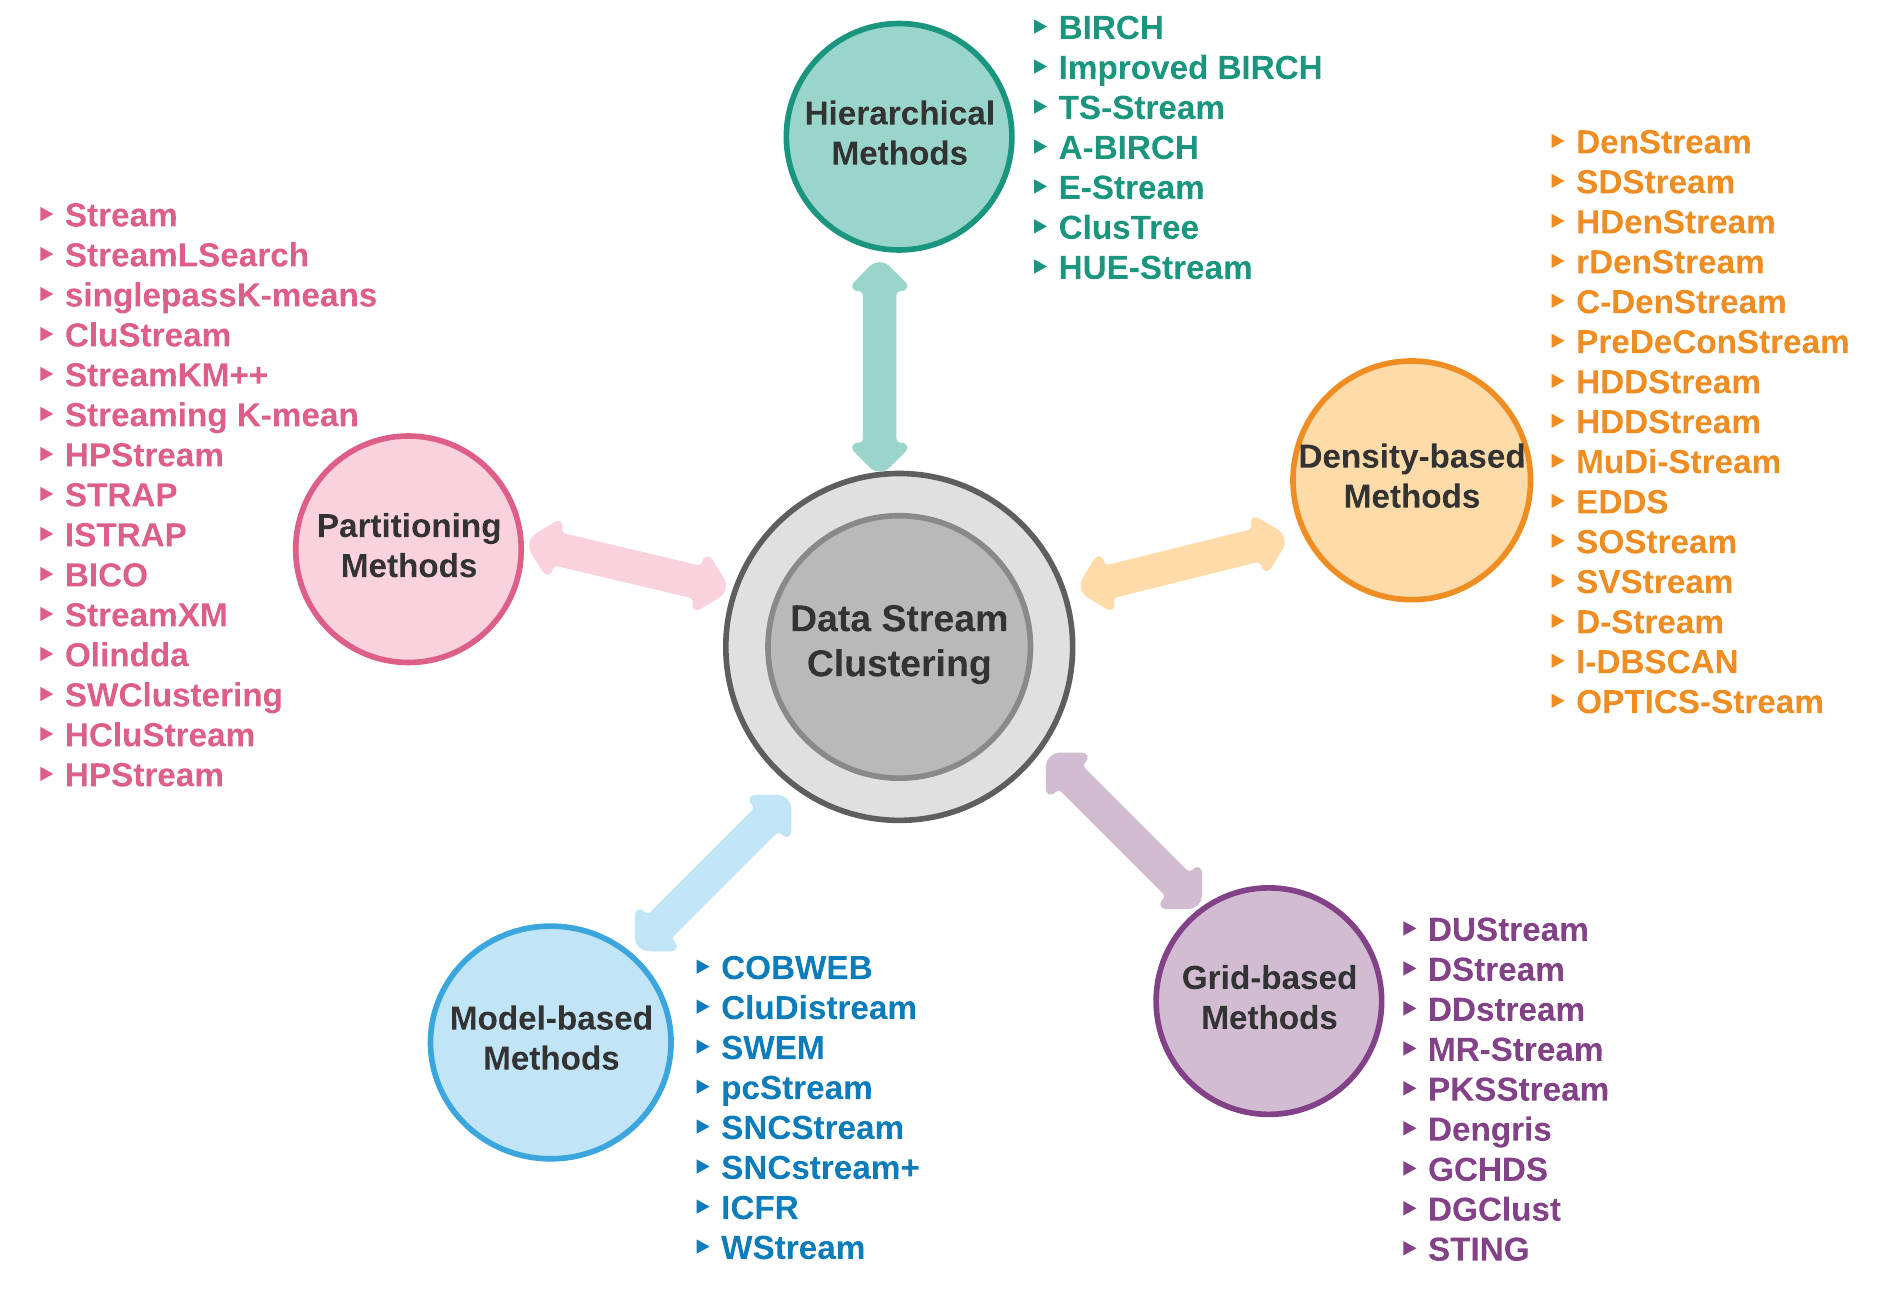
\includegraphics[width = 12 cm]{image/Chapters/Chapter2/streammethod.png}
\caption{Data stream clustering methods and algorithms.}
\label{method}
\end{figure}


% \begin{itemize}
%     \item\textit{Streaming Partitioning Methods:} Table \ref{landmarkwin} provides an overview of the main methods proposed for updating the partitioning process of stream data points using landmark, sliding, and pyramidal time windows. 


%The First group is partitioning data stream clustering algorithm, which is listed in Table Table \ref{landmarkwin}. 
%As far as we had researched, no research work with affinity propagation used landmark time window model is presented.



\begin{table}[!ht]
\centering
\small
\caption{Overview of data stream clustering methods \protect\cite{mansalis2018evaluation}}
\label{landmarkwin}
\begin{tabular}{lllll}
\hline
\textbf{Algorithms} & \textbf{Year} & \textbf{Approach} & \textbf{Processing} & \textbf{Time Window} \\ \hline \midrule
\multicolumn{5}{c}{\cellcolor[HTML]{C0C0C0}\textbf{Partitioning-based}}                              \\ \hline
Stream              & 2000          & k-median          & Single-pass         & Landmark             \\ \hline
StreamLSearch       & 2002          & k-median          & Single-pass         & Landmark             \\ \hline
CluStream           & 2003          & k-means           & Online-Offline      & Pyramidal            \\ \hline
HCluStream          & 2006          & k-means           & Online-Offline      & Pyramidal            \\ \hline
Olindda             & 2007          & k-means           & Online-Offline      & Landmark             \\ \hline
SWClustering        & 2008          & k-means           & Online-Offline      & Sliding              \\ \hline
StreamKM++          & 2012          & k-means++         & Online-Offline      & Landmark             \\ \hline
BICO                & 2013          & k-means           & Online-Offline      & Landmark             \\ \hline
StreamXM            & 2015          & x-means           & Merge-reduce        & Landmark             \\ \hline
\multicolumn{5}{c}{\cellcolor[HTML]{C0C0C0}\textbf{Hierarchical-based}}                              \\ \hline
BIRCH               & 1996          & CF-tree           & Single-pass         & Landmark             \\ \hline
TS-Stream           & 2015          & Decision Tree     & Single-pass         & Sliding              \\ \hline
\multicolumn{5}{c}{\cellcolor[HTML]{C0C0C0}\textbf{Density-based}}                                   \\ \hline
DenStream           & 2006          & DBSCAN            & Online-Offline      & Damped               \\ \hline
SDStream            & 2009          & DBSCAN            & Online-Offline      & Sliding              \\ \hline
HDenStream          & 2009          & DBSCAN            & Online-Offline      & Damped               \\ \hline
FlockStream         & 2009          & Swarms            & Single-pass         & Damped               \\ \hline
rDenStream          & 2009          & DBSCAN            & Online-Offline      & Damped               \\ \hline
C-DenStream         & 2009          & C-DBSCAN          & Online-Offline      & Damped               \\ \hline
PreDeConStream      & 2012          & DBSCAN            & Online-Offline      & Damped               \\ \hline
HDDStream           & 2012          & DBSCAN            & Online-Offline      & Damped               \\ \hline
MuDi-Stream         & 2016          & DBSCAN            & Online-Offline      & Damped               \\ \hline
EDDS                & 2017          & DBSCAN            & Online-Offline      & Damped               \\ \hline
\multicolumn{5}{c}{\cellcolor[HTML]{C0C0C0}\textbf{Grid-based}}                                      \\ \hline
DUstream            & 2005          & Dense-unit        & Online-Offline      & Landmark             \\ \hline
D-stream            & 2007          & Dense-region      & Online-Offline      & Damped               \\ \hline
DDStream            & 2008          & DCQ-means         & Online-Offline      & Damped               \\ \hline
MR-Stream           & 2009          & Dense-region      & Online-Offline      & Damped               \\ \hline
PKS-Stream          & 2011          & Dense-region      & Online-Offline      & Damped               \\ \hline
DENGRIS             & 2012          & Dense-region      & Single-pass         & Sliding              \\ \hline
\multicolumn{5}{c}{\cellcolor[HTML]{C0C0C0}\textbf{Model-based}}                                     \\ \hline
COBWEB              & 1987          & Tree-based        & Online-Offline      & Landmark             \\ \hline
SWEM                & 2009          & EM Algorithm      & Online-Offline      & Sliding              \\ \hline
pcStream            & 2015          & SIMCA             & Single-pass         & Damped               \\ \hline
SNCStream           & 2015          & Network           & Online              & Damped               \\ \hline
SNCStream+          & 2016          & Network           & Online              & Damped               \\ \hline \midrule
\end{tabular}
\end{table}












% \begin{table}[h]
%     \centering
%     \caption{ Overview of data stream clustering methods \protect\cite{mansalis2018evaluation}}
%     \label{landmarkwin}
%     \small
%     \begin{tabular}{c c c c c}
%     \hline
%       \normalsize{\textbf{Algorithms} & \textbf{Year} & \textbf{ Approach } & \textbf{Processing} & \textbf{ Time Window}}  \\
%      \hline \midrule
%       \rowcolor{lightgray}& &\rowcolor{lightgray}\centering \textbf{Partitioning-based }  & &  \\
%       \hline 
%       \hline
%       Stream             &   2000    &   k-median     &  Single-pass       & Landmark \\
%      \hline
%       StreamLSearch      &   2002    &   k-median     &   Single-pass      & Landmark \\
%     \hline
%      CluStream           &   2003    &  k-means       &  Online-Offline    & Pyramidal \\
%     \hline   
%      HCluStream         &    2006   &    k-means     & Online-Offline      & Pyramidal \\
%     \hline
%      Olindda            &   2007    &   k-means      &   Online-Offline    & Landmark  \\
%     \hline    
%      SWClustering        &    2008   &    k-means     &  Online-offline    & Sliding   \\
%       \hline
%       StreamKM++         &    2012   &   k-means++    & Online-Offline     & Landmark   \\
%     \hline 
%       BICO               &    2013   &    k-means     &  Online-Offline    & Landmark  \\
%       \hline
%       StreamXM           &    2015   &    X-means     &  Merge-reduce    & Landmark  \\
%         \hline
%       \hline
%       \rowcolor{lightgray}&& \rowcolor{lightgray}\centering\textbf{Hierarchical-based }  & &  \\
%       \hline 
%       \hline 
%       BIRCH             &    1996        &     CF-tree           &  Single-pass    & Landmark \\
%      \hline
%       TS-Stream         &     2015       &    Decision Tree      & Single-pass     & Sliding  \\
%       \hline
%       \hline
%      \rowcolor{lightgray}& &\rowcolor{lightgray}\centering \textbf{Density-based}  & &  \\
%       \hline 
%       \hline
%     DenStream            &    2006     &    DBSCAN       & Online-offline  &   Damped   \\
%      \hline
%      SDStream            &    2009     &    DBSCAN       & Online-offline  &   Sliding \\
%       \hline
%       HDenStream         &     2009    &    DBSCAN       &  Online-offline &   Damped  \\
%         \hline
%       FlockStream        &     2009    &    Swarms       &  Single-pass    &   Damped  \\
%         \hline 
%       rDenStream         &    2009     &     DBSCAN      & Online-offline  &   Damped  \\
%         \hline 
%       C-DenStream        &    2009     &     C-DBSCAN    &Online-offline   &   Damped \\
%           \hline 
%       PreDeConStream     &    2012     &     DBSCAN      & Online-offline  &   Damped \\
%           \hline 
%       HDDStream          &    2012     &     DBSCAN      & Online-offline  &   Damped   \\
%           \hline 
%       MuDi-Stream        &    2016     &       DBSCAN    & Online-offline  &   Damped\\
%       \hline          
%       EDDS               &    2017     &     DBSCAN      & Online-offline  &   Damped \\
%       \hline
%       \hline
%      \rowcolor{lightgray}& &\rowcolor{lightgray}\centering \textbf{Grid-based}  & &  \\
%       \hline 
%       \hline      
%      DUstream            &    2005        &      Dense-unit       &     Single-pass    &  Landmark\\
%       \hline
%       D-stream           &     2007       &    Dense-region       &  Online-offline    &   Damped\\
%     \hline 
%       DDStream           &    2008        &    DCQ-means          &     Online-offline & Damped \\
%     \hline 
%       MR-Stream          &    2009        &     Dense-region      &  Online-offline    & Damped\\
%     \hline 
%       PKS-Stream         &    2011        &    Dense-region       &  Online-offline    & Damped\\
%     \hline 
%       DENGRIS            &    2012        &   Dense-region        &  Single-pass       & Sliding\\
%       \hline 
%       \hline
%      \rowcolor{lightgray}& &\rowcolor{lightgray}\centering\textbf{Model-based}  & &  \\
%       \hline 
%       \hline
%       COBWEB             &    1987        &   tree-based      &    Online-offline   & Landmark \\
%      \hline
%       SWEM               &    2009        &  EM Algorithm     &  Online-offline     & Sliding\\
%      \hline
%      pcStream            &    2015        &    SIMCA          &   Single-pass       & Damped  \\
%     \hline 
%       SNCStream          &    2015        &    Network        &   Online            & Damped  \\
%     \hline 
%     SNCStream+      &    2016        &       Network     &    Online           & Damped  \\
      
% \bottomrule
%     \end{tabular}
% \end{table}

In this research work, the DSAP algorithm is proposed as a simplification of the previous streaming AP algorithms. This is further discussed in the next Chapter.


% In particular, the online-offline processing for streaming K-means clustering has been applied to many algorithms such as CluStream, Olindda, SWClustering, and BICO. The open-source available DSC\_TwoStage in R version of streaming K-means using the 2-phase processing was used in this thesis, and is further discussed in Chapter 5.  



% The Stream algorithm proposed by Guha et al. \cite{o2002streaming} is one of the earliest approaches in this field. This method is the k-median approach and divides the stream into batches of data with a fixed size. At each batch, the k-median algorithm is applied. 


% Olindda introduced by Spinosa \cite{spinosa2007olindda}, based on the K-means clustering algorithm, is an online anomaly detection algorithm. Olindda continuously monitors and adapts to emerging data distributions. Unknown samples are kept in a memory queue and are periodically clustered and then either merged with an existing similar cluster or added as a novel cluster to the pool of clusters.
% This model calculates the maximum distance between data points and centroids as a decision boundary (threshold) for each cluster. The union of the boundaries of all clusters is the global decision boundary that defines the model. A new unseen data point that falls inside this boundary is consistent with the model and therefore considered normal. Otherwise, This specific data point is labeled as an unknown and separated for further analysis.
% %similar to my work
% CluStream \cite{aggarwal2003framework} is inherited from the BIRCH algorithm. The online phase is started by applying the k-means algorithm to create micro-clusters. When a new data point arrives, it is absorbed by its closest micro-cluster if it fit within an adaptive radius threshold. Otherwise, it creates a new cluster. To keep micro-clusters in some range, expired clusters are removed based on a threshold on their average time stamp. If it cannot happen, the two closest micro-clusters will be merged.
% To support different time-horizons, CluStream frequently collects snapshots of the current CFs by a pyramidal time frame. 

% Another algorithm is HCluStream \cite{yang2006hclustream} is an extension of CluStream for categorical data by storing the frequency of attribute-levels for all categorical features. This algorithm creates a  categorical distance measure separately to combine with the traditional distance measure for continuous attributes.

% SWClustering \cite{zhou2008tracking} introduced a new data structure for this algorithm called Exponential Histogram of Cluster Feature (EHCF), which can handle cluster evolution and represents the changes of the cluster distribution and capture it. In the online phase, it captures objects as synopses in the EHCF structure, and in the offline phase, the algorithm clusters these collections of synopses using a k-means algorithm.

% Ackermann et al. \cite{ackermann2012streamk} develop a new coreset construction for the Euclidean k-means clustering problem and called it StreamKM++. A coreset is a small weighted point set that approximates the original input point set with respect to a given optimization problem. This algorithm proposed a coreset construction for the Euclidean k-means clustering problem called coreset tree suitable for high dimensional data. Then, they used a standard streaming technique, called the merge-and-reduce technique, to maintain observation in data streams. After processing the whole input stream, the k-MEANS++ algorithm applies to obtain a k-means clustering and celled it the StreamKM++ algorithm.

% BICO \cite{fichtenberger2013bico} is another algorithm in this group that combines the BIRCH data structure with StreamKM++. 






%\item\textbf{Hierarchical-based algorithms:}

% \begin{table}[h]
%     \centering
%     \caption{Overview of Hierarchical-based stream clustering algorithms. }
%     \label{hirarcha}
%     \small
%     \begin{tabular}{c c c c c}
%     \hline
%       \textbf{Algorithms} & \textbf{Year} & \textbf{ Method } & \textbf{Processing} & \textbf{ Time Window}  \\
%      \hline \midrule

%       BIRCH             &    1996        &     CF-tree  &         & Landmark \\
%      \hline
%      Improved BIRCH     &    2014        &    CF-tree   &         & Landmark \\
%       \hline
%       TS-Stream         &     2015       &    -      &       & Sliding  \\
%     \hline 
%       A-BIRCH           &    2017        &   CF-tree    &      & Landmark\\
% \bottomrule
%     \end{tabular}
% \end{table}

%BIRCH \cite{zhang1996birch} is one of the earliest stream clustering algorithms. This algorithm minimizes large datasets' memory requirements by summarizing the information contained in dense regions as Clustering Feature (CF) entries. CF has three components: the number of data points, the d-dimensional vector with the linear sum of all data points, and a sum of squares for all data points across dimensions. BIRCH incrementally builds a balanced-tree to maintain CFs, where each node can contain a fixed number of CFs. 
%For every new data point that comes into the model, the tree descends by following the child to its closest CF until a leaf node is reached. The new data point can either merged to its closest leaf-CF or creates a new leaf-CF. This method has a significant drawback which is the limited capacity of its leaves.

% Improved BIRCH \cite{ismael2014improved} is an extension of the BIRCH algorithm, which employs various distance thresholds per CF.

% TS-Stream \cite{pereira2014ts} is a time-series data stream clustering with the time frame. 

% A-BIRCH \cite{lorbeer2016birch} is similar to Improved BIRCH, determines the threshold parameters by using the Gap Statistics on a representation of the stream.



% \item\textbf{Density-based algorithms:}

% \begin{table}[h]
%     \centering
%     \caption{Overview of Density-based stream clustering algorithms. }
%     \label{densalgo}
%     \small
%     \begin{tabular}{c c c c c}
%     \hline
%       \textbf{Algorithms} & \textbf{Year} & \textbf{ Time window } & \textbf{Method} & \textbf{ Processing}  \\
%      \hline \midrule

%       DenStream          &    2006        &    Damped          &    DBSCAN      & Online-offline \\
%      \hline
%      SDStream            &    2009        &    Sliding         &    DBSCAN      & Online-offline \\
%       \hline
%       HDenStream         &     2009       &     Damped         &    DBSCAN      &  Online-offline \\
%         \hline 
%       rDenStream         &    2009        &    Damped         &     DBSCAN      & Online-offline \\
%         \hline 
%       C-DenStream        &    2009        &    Damped         &     C-DBSCAN    &Online-offline \\
%           \hline 
%       PreDeConStream     &    2012        &   Damped          &     DBSCAN      & Online-offline\\
%           \hline 
%       HDDStream          &    2012        &   Damped          &     DBSCAN      & Online-offline\\
%           \hline 
%       EDDS               &    2017        &   Damped          &     DBSCAN      & Online-offline\\
% \bottomrule
%     \end{tabular}
% \end{table}

% DenStream \cite{cao2006density} is the temporal extension of the CFs from the BIRCH algorithm with having core micro cluster using time-faded CF. This algorithm was implemented with arbitrary shape data.

% SDStream \cite{ren2009density} is a variant of DenStream algorithm for sliding time window model. This algorithm keeps CMCs in the form of an Exponential Histogram.
 
% HDenStream \cite{lin2009density} is a combination of DStream (with the categorical distance measure ) and HCluStream for categorical datasets. 

% FlockStream \cite{forestiero2013single} applies a flocking behavior to identify emerging flocks and swarms of objects. Like the DenStream algorithm, FlockStream differentiates between potential core and outlier micro-clusters and uses a time-faded CF. 

% rDenStream \cite{liu2009rdenstream} to detects outliers,  this algorithm temporarily stores them away in an outlier buffer.  After the offline phase, the algorithm tries to re-cluster the data points cached in the buffer to improve the clustering.

% C-DenStream \cite{ruiz2009c} is another type of  DenStream that allows domain knowledge in instance-level constraints into the clustering method. Instance-level constraints mean data points that can or cannot belong to the same cluster.

% PreDeConStream \cite{hassani2012density} was implemented simultaneously to HDDStream. The algorithm changes in regular intervals by applying a modified PreDeCon algorithm on the micro-clusters generated during the online phase.

% HDDStream \cite{ntoutsi2012density}

% \item\textbf{Grid-based algorithms:}
% Grid-based algorithms capture the density in the grid. Macro-clusters are usually obtained by grouping adjacent dense cells. How to make a grid cell is very challenging. Table \ref{gridd} shows the overview of some main algorithms in this group. The most popular grid-based algorithm is DStream \cite{chen2007density}.


% \begin{table}[h]
%     \centering
%     \caption{Overview of grid-based stream clustering algorithms. }
%     \label{gridd}
%     \small
%     \begin{tabular}{c c c c c}
%     \hline
%       \textbf{Algorithms} & \textbf{Year} & \textbf{ Method } & \textbf{Processing} & \textbf{ Time Window}  \\
%      \hline \midrule

%       Fractal Clustering &    2000        &                       &  Online            &   Landmark\\
%           \hline 
%      DUstream            &    2005        &      Dense-unit       &     Online         &  Landmark\\
%       \hline
%       Dstream            &     2007       &    Dense-region       &  Online-offline    &   Damped\\
%     \hline 
%       DDStream           &    2008        &    DCQ-means          &     Online-offline & Damped \\
%     \hline 
%       MR-Stream          &    2009        &     Dense-region      &  Online-offline    & Damped\\
%     \hline 
%       PKS-Stream         &    2011        &    Dense-region       &  Online-offline    & Damped\\
%           \hline 
%       DENGRIS            &    2012        &   Dense-region        &  Online            & Sliding\\
%           \hline 
%       HDCStream          &    2014        &                       &    Online          & Damped\\
%           \hline 
%       MuDi-Stream        &    2016        &       DBSCAN          & Online-offline      & Damped\\
% \bottomrule
%     \end{tabular}
% \end{table}

% Dstream has a fixed grid size, with three different types of cells: dense cells, sparse cells, and transitional cells, which it is categorized between the other two types. The algorithm outlines new data points to its corresponding cell and is initialized by assigning all dense cells to individual clusters. These clusters are extended with all neighboring transitional grids or merged with neighboring dense cell clusters. In any intervals, the clustering assesses the weight of individual cell and includes the
% changes in cell types into the clustering.


% DUstream \cite{gao2005incremental} devides the data space once into fixed grid-cells.
% The algorithm processes the first part of data to start the clustering and maintains all cells with sufficient density. The density of cells is determined, corresponding to the total number of observations. 

% DDstream \cite{jia2008grid} is an extension of points that lie precisely on the grid boundaries. For these points, the distance to adjacent cell centers is calculated, and those points are assigned to their closest cell. 





% \item\textbf{Model-based algorithms:}
% This group of algorithms summarize the data stream as a statistical model, usually based on Expectation Maximization (EM) algorithm. 

% \begin{table}[h]
%     \centering
%     \caption{Overview of model-based stream clustering algorithms. }
%     \label{modealgo}
%     \small
%     \begin{tabular}{c c c c c}
%     \hline
%       \textbf{Algorithms} & \textbf{Year} & \textbf{ Method } & \textbf{Processing} & \textbf{ Time Window}  \\
%      \hline \midrule

%       COBWEB             &    1987        &   tree-based   &          & Landmark \\
%      \hline
%      WStream             &    2004        &   Kernel-density  &                     & Damped \\
%       \hline
%       CluDistream        &     2007       &   EM           &        &  Landmark \\
%     \hline 
%       SWEM               &    2009        &  EM            &  Online-offline      & Sliding\\
%     \hline 
%       SVStream          &    2013         &    SVC         &                     & Damped  \\
%     \hline 
%       pcStream          &    2015         &       SIMCA    & Online        & Damped  \\
% \bottomrule
%     \end{tabular}
% \end{table}


% COBWEB \cite{fisher1987knowledge} is a tree-based algorithm, and each node describes a cluster. Tree incrementally builds by descending a new entry from the root to a leaf. 

% WStream \cite{tasoulis2006unsupervised} uses kernel density to keeps several windows in the data space. It means to use the local maxima of a density estimate as cluster centers and the local minima as cluster boundaries. New data points can add to an existing window, or it is used to initialize a new window with the default size. 

% CluDiStream \cite{zhou2007distributed} applies EM algorithm for data stream clustering. This algorithm learns the distribution of underlying data streams by maximizing the likelihood of the data clusters. It keeps the distribution of Gaussian mixture and a coordinator node in each location to combine the distributions.

% SWEM \cite{dang2009based} uses EM to chunks of data with random initial parameters. Distributions for the first chunk of data calculates. Each cluster is then summarized using a CF and macro-clusters by applying EM again.

% SVStream \cite{wang2011svstream} is based on support vector clustering (SVC), which transforms the data into the higher dimensional space. The model is run in chunks, and the first one runs SVC. For other chunks, it checks if it is in the radius of spheres or not. If yes, a new sphere is initialized. 






% \end{itemize}

% \subsection{Streaming k-means clustering}

% move things from the other chapters(s) to here
% look at the thesis from Luke to describe the method. the only [platform we have is R]
   	    
% Streaming clustering with K-means is employed to provide fast responses where new data points coming into the data stream are analyzed near real-time instead of applying as an traditional K-means method for a particular dataset. Different type of stream clustering with K-means are available during the history of stream clustering. 

% to keep the clustering computational effort beyond reasonable limits for large-scale data in an online fashion, divide and conquer approach is deployed by using K-means traditional algorithm \cite{nittel2004scaling}. 
% This approach has mainly three steps as shown in Figure \ref{dividee}: partitioning the dataset into different chunks, then clustering each chunk and find the results, lastly, computes the results out of all chunks of data. 

% \begin{figure}[!h]
%     \centering
%     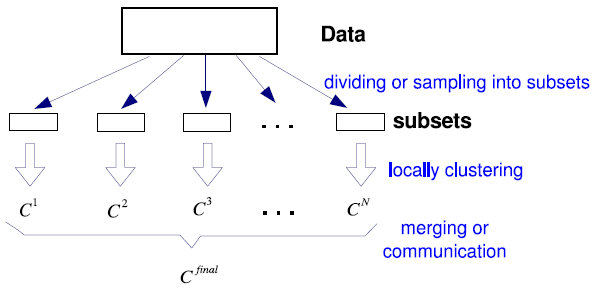
\includegraphics[width = 11 cm]{image/Chapters/Chapter3/divide.PNG}
%     \caption{Divide and conquer approach to generate clustering out of big data \protect\cite{zhang2009toward}}
%     \label{dividee}
% \end{figure}   	    
% \cite{khalilian2016data} 
% The query processing cost for such a method is high, and it does not work for applications that require fast query response. Remarkably, they require merging multiple data structures at the time of query, followed by an extraction of cluster centers, which is expensive \cite{zhang2017streaming}.

% The online and offline streaming K-means clustering approach has applied on different algorithms such as CluStream, Olindda, SWClustering, BICO. 



% The open-source available version of streaming K-means is DSC\_TwoStage in R programming language. 




% \begin{algorithm}[H]
% \SetAlgoLined
% \textbf{Input:} Data stream $S=(s_{1}, s_{2},...,s_{n})$, number of micro clusters $k$, number of macro cluster $k_m$, sliding time window $W$ with the size $z$;\\
% \textbf{Output:} {Set of micro clusters $C_m= (C_{m_1}, C_{m_2}, ..., C_{m_k})$, and set of macro clusters $C_M= (C_{M_1}, C_{M_2}, ..., C_{M_{k_m}})$ }\\
% \SetKwFunction{FIROC}{Streaming K-means}
% \SetKwProg{Fn}{Function}{:}{}
% \Fn{\FIROC{S, W}}{
         
% \textbf{Initialization:}
% \begin{itemize}
%     \item Partition S with $W$ into k subsets $S_1$, . . . , $S_k$, such that $S_i$, 1 $\leq$ i $\leq$ k,
%     \item Extract $W_1$ = $(s_1...s_z)$ data points from $S$
%     % \item partition S with $W$ into k subsets $S_1$, . . . , $S_k$
%     \item Estimate $k$ initial centroids $c_1, . . . , c_k$ from $W_1$ using K-means
% \end{itemize}

% \Repeat{Centroid convergence is achieved}{          
%  \SetKwFunction{FIROC}{K-means}         \hfill \Comment{Online Phase}\\
% \SetKwProg{Fn}{Function}{:}{}
% \Fn{\FIROC{Wi,k}}{
%  Assign data points $s_i$ to the closest centroid\\
%  Replace the current centroids by new centroids $c_1, ..., c_i$\\}
% \textbf{return}{ $(C_{m_1}, C_{m_2}, ..., C_{m_k})$ }\\
% }

% \Repeat{Centroids convergence happens}{
%   \SetKwFunction{FIROC}{K-means}         \hfill \Comment{Offline Phase}\\
% \SetKwProg{Fn}{Function}{:}{}
% \Fn{\FIROC{C_m,k_m}}{                                     
%   Find $k_m$ macro clusters from $C_m$ centroids\\
%   }
% }

% \textbf{return} {macro clusters: $C_{M_1}, C_{M_2}, ..., C_{M_{k_m}}$\\ }
% }
%  \caption{Streaming K-means Online Micro and Offline Macro Clustering Algorithm}
% \end{algorithm}


%New ideas continue evolving in data streams over time. Evolving needs updating data stream algorithms to adjust to the changes such as handle well rapid cluster evolution patterns.







%%%%%%%%%%%%%%%%%%%%%%%%%%%%%%%%%%%%%%%%%%%%%%%%%%%%%%chapter 4
% \section{online- offline clustering}
% This section introduced a three phase, online micro, offline macro, and evaluation streaming K-means algorithm for comparison with the proposed DSAP algorithm. The streaming K-means algorithms are  widely used to analyze streaming data. In this section, the framework of streaming K-means algorithm is discussed. As shown earlier in Figure \ref{wrk1} the DSAP and streaming K-means algorithms have analogous phases with the major differences in the clustering algorithm.
% \subsection{Online Micro-Clustering Phase}
% In this phase, the data stream arrives are accumulated using the sliding time window model. The streaming K-means model incrementally updates when a new data window comes into the model to generate the micro clusters. These points can also be clustered using K-means with preferred $k$ cluster centroids. The approach used for selecting the $k$ number of micro clusters is the elbow method described previously in section \ref{elbowmethod}. The algorithm randomly chooses $n$ data points in each time frame until convergence happens. It computes the sum of the squared distances from each data point to its assigned centroid.

% \begin{figure}
% \centering
% 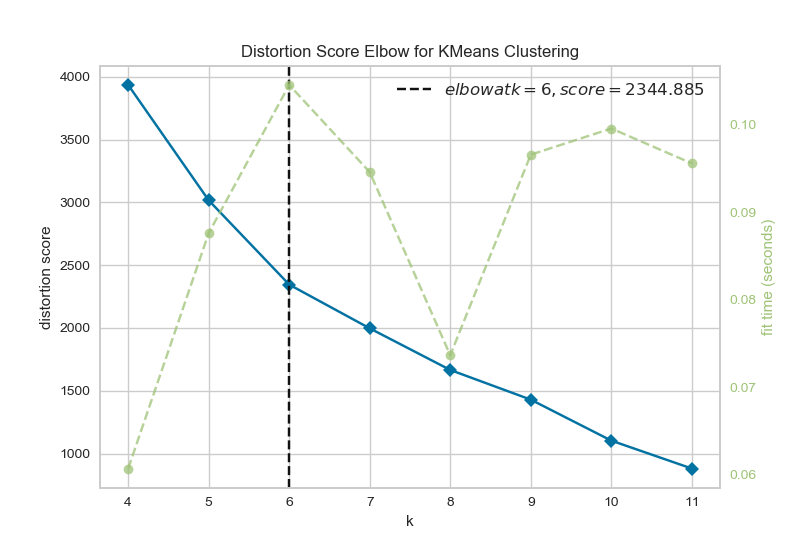
\includegraphics[width = 12cm,height = 8cm]{image/elbow.png}
% \caption{The elbow curve found for a $k$ range from 4 to 11 clusters. The black dotted line is the number of clusters determined by the elbow method}
% \label{elb}
% \end{figure}




%\subsection{Streaming K-means Clustering Performance Evaluation}
%The quality and efficiency of the streaming K-means clustering algorithm need to be evaluated as well as the DSAP algorithm. The quality of clusters found by each algorithm are assessed by these four criteria: Silhouette Coefficient, Calinski-Harabasz Index, Davies-Bouldin Index and outlier detection.
%The efficiency is compared using three metrics: computational time efficiency, frequency of the outliers and the memory consumed to run the program.



%\subsubsection{Evaluation of Data Stream Clustering}

%In data stream clustering (DSC) phase, stream currently provides moving windows and sampling from a stream as data stream operators.DSC\_Window provides a clustering interface to the data stream. It implements the sliding window and the dampened window models which keep a user-specified number (window length) of the most recent data points of the stream. For the dampened window model, data points in the window have a weight that deceases exponentially with age.
%%%elmi
%Evaluating the performance of a clustering algorithm is not counting the number of errors or accuracy. In particular, any evaluation metric if this clustering defines separations of the data similar to some ground truth set of classes or satisfying some assumption such that members belong to the same class are more similar than members of different classes according to some similarity metric.The main purpose of clustering methods is to find high intra-cluster similarity and low inter-cluster similarity. In a simple term, objects in the same cluster are more similar than the objects in different clusters.
%%




%%%%%%%%%%%%%%%%%%%%%%%%%%%%%%%%%%%%%%%%%%%%%%%%%%%%%%%%%%%%%%%%%%%%%%%%%%%%%%% KEEP
% \section{Sliding Time Window Model}
% The sliding time window model limits the scope of data to a sequence of the most recent data points in the data stream to compute the micro clusters, since the new data point is available, the old one is removed.
% The first window is started with a pre-defined time frame based on the data, and this window containing the accumulated data points from where the stream started. After a new data point arrives, the algorithm updates the micro clusters incrementally each time. Next, the new time window employs all the new data points and clusters as the data points, saving the new micro clusters and the selected centroids. 

% By applying a sliding time window model, the sum of square distances will often eliminate at a local optimum. Accordingly, it leads to the micro-clustering evolution results. The main focus is finding micro clusters evolution to identify new clusters from outliers. There are two types of sliding windows, time-based and count-based sliding windows \cite{li2014parallel}. In time-based sliding windows, time intervals are applied(e.g., every 10 minutes), while in count-based sliding windows, they are defined in terms of the number of data points. Figure \ref{stw} shows sliding time window model with the data points included in a window.  Equation \ref{eq11} shows the calculation of time window:
% \begin{equation}
%     W_i = [m_i, ..., m_{(i+w-1)}]\label{eq11}
% \end{equation}

% Where $w$ is a window length, $m_i$ is the $i^{th}$ data point and $W_i$ is the $i^{th}$ window. 
% \begin{figure}
% \centering
% %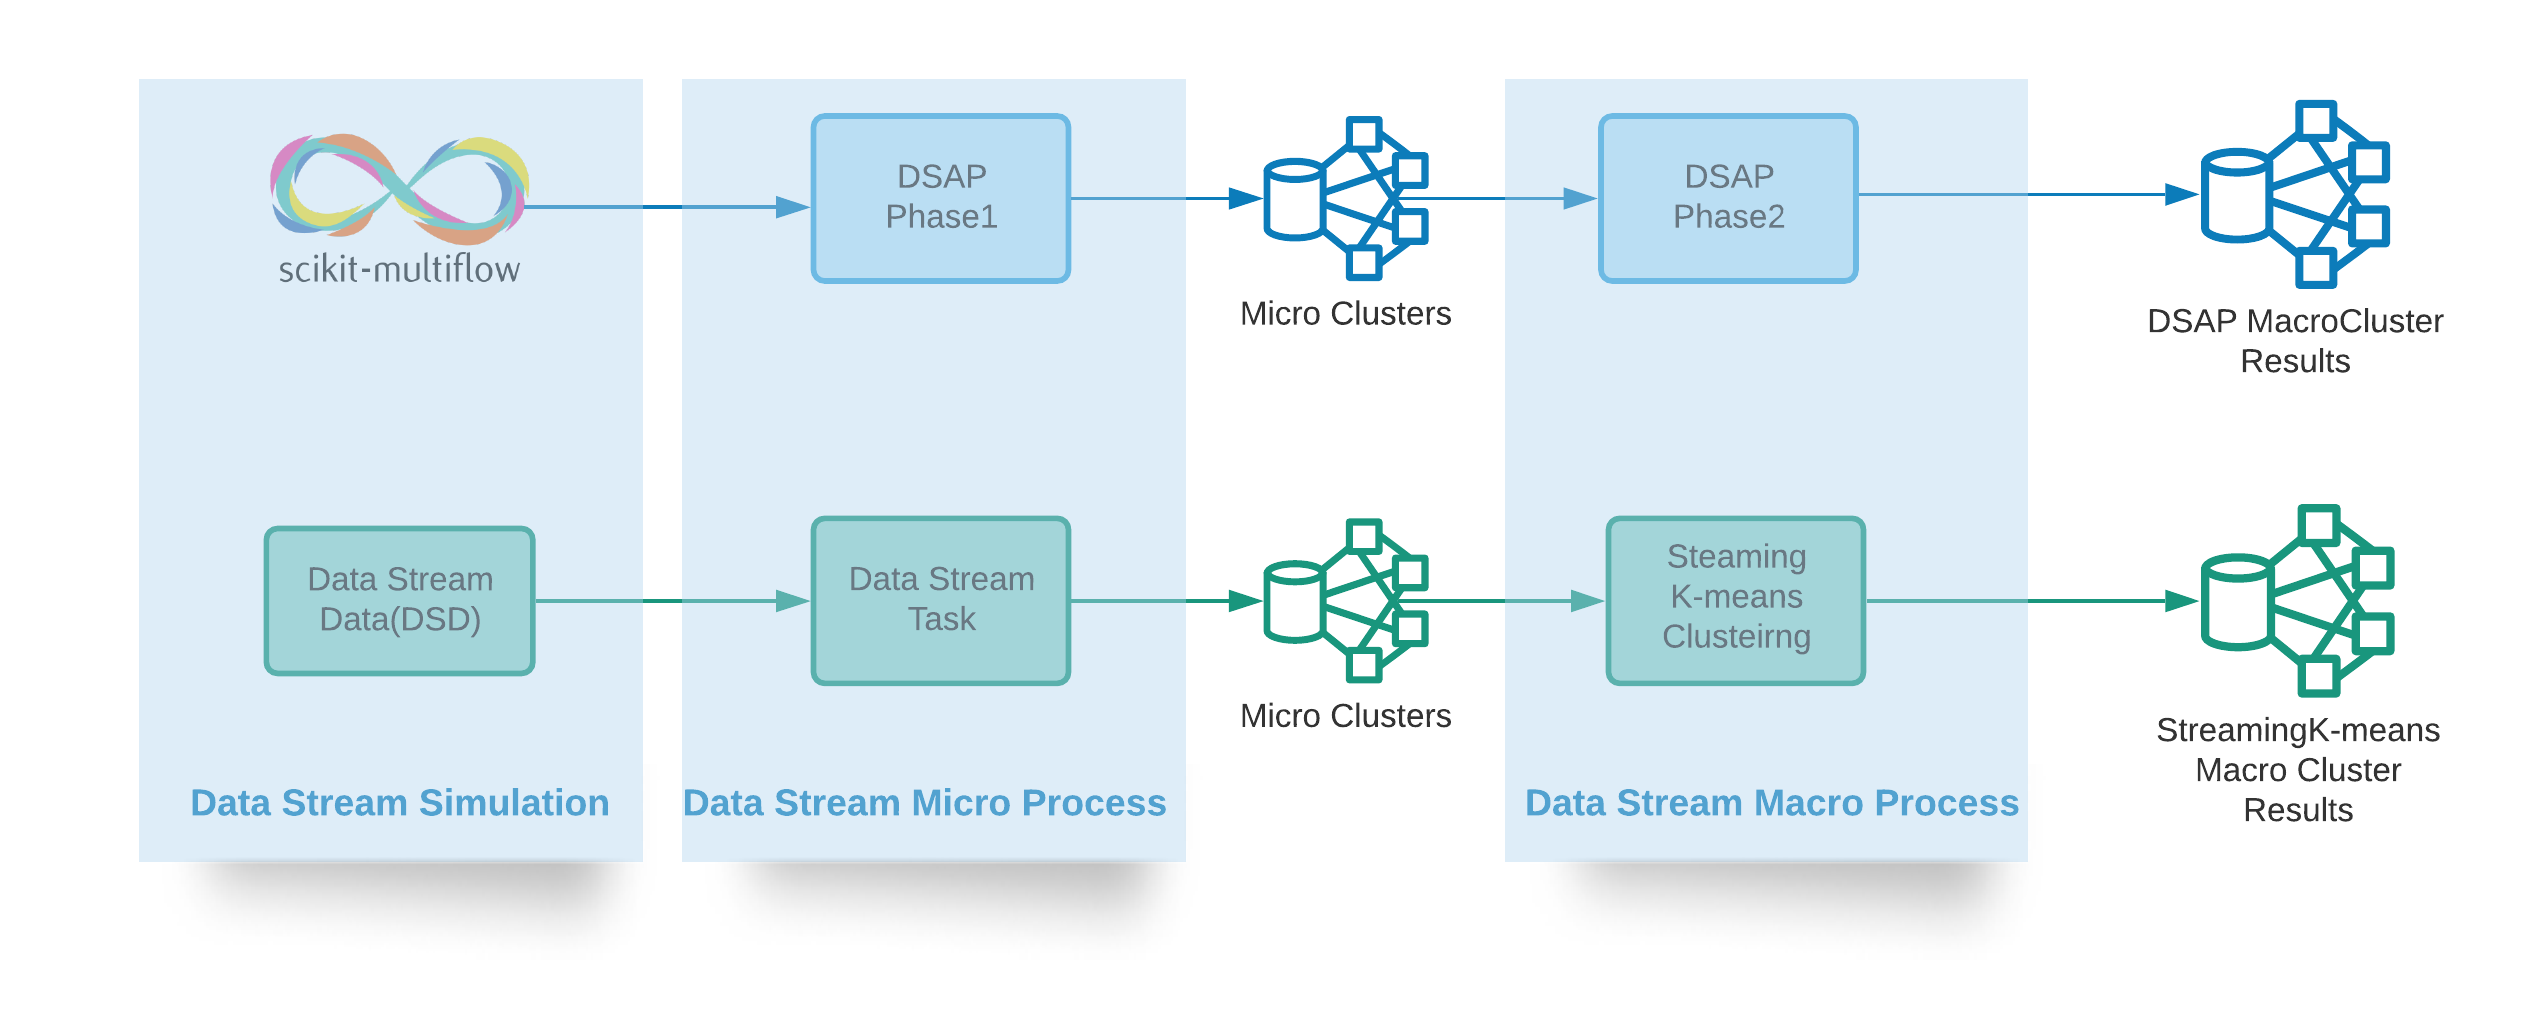
\includegraphics[width = 15cm,height = 7cm]{image/2-2workflow.png}
% 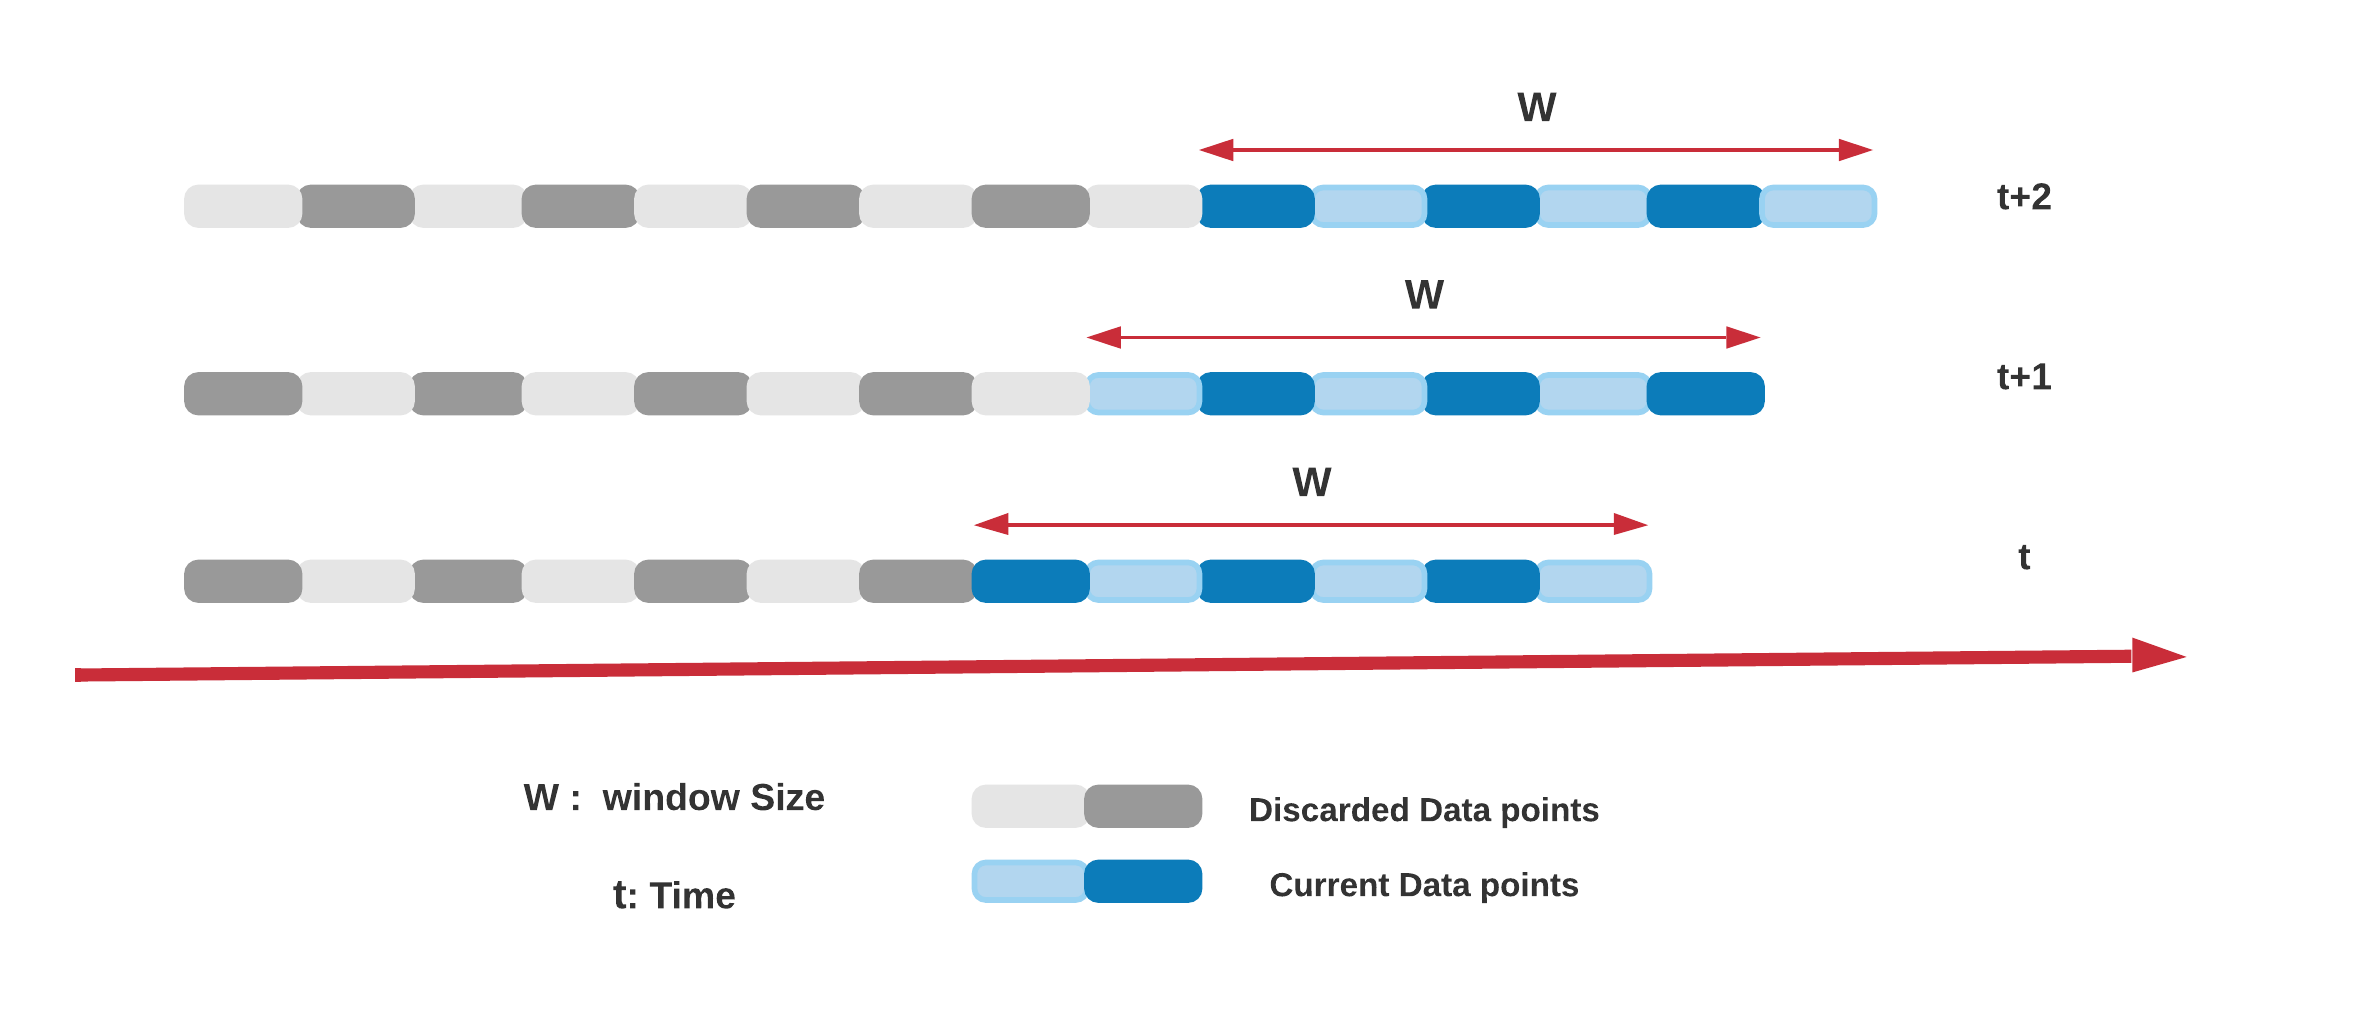
\includegraphics[width = 14cm,height = 7cm]{image/stw (2).png}
% \caption{Sliding time window model applied in this work\cite{zubarouglu2020data}}
% \label{stw}
% \end{figure}
% \cite{zubaroglu2020data}









%%%%%%%%%%%%%%%%%%%%%%%%%%%%%%%%%%%%%%%%%%%%%%%%%%%%%%%%%%%%%%%%%%%%%%%%%%%%%%%%%%





% \begin{figure}
% \centering
% 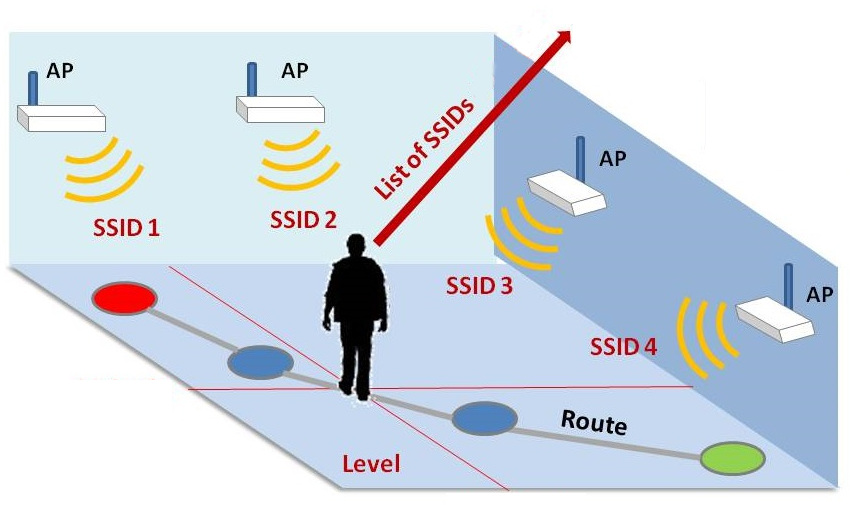
\includegraphics[width = 9cm,height = 6cm]{image/indoorp.jpg}
% \caption{Indoor positioning technique using WLAN . }
% \label{time}
% \end{figure}

%elmi


%elmi. RSSI, or “Received Signal Strength Indicator,” is a measurement of how well your device can hear a signal from an access point or router.  RSSI is a term used to measure the relative quality of a received signal to a client device, but has no absolute value. The IEEE 802.11 standard (a big book of documentation for manufacturing WiFi equipment) specifies that RSSI can be on a scale of 0 to up to 255 and that each chipset manufacturer can define their own “RSSI Max” value. Cisco, for example, uses a 0-100 scale, while Atheros uses 0-60. Since RSSI varies greatly between chipset manufacturers,

%elmi. wiki.In an IEEE 802.11 system, RSSI is the relative received signal strength in a wireless environment, in arbitrary units. RSSI is an indication of the power level being received by the receiving radio after the antenna and possible cable loss. Therefore, the greater the RSSI value, the stronger the signal. Thus, when an RSSI value is represented in a negative form (e.g. −100), the closer the value is to 0, the stronger the received signal has been. There is no standardized relationship of any particular physical parameter to the RSSI reading. The 802.11 standard does not define any relationship between RSSI value and power level in milliwatts or decibels referenced to one milliwatt (dBm). Vendors and chipset makers provide their own accuracy, granularity, and range for the actual power (measured as milliwatts or decibels) and their range of RSSI values (from 0 to RSSI maximum).[2] One subtlety of the 802.11 RSSI metric comes from how it is sampled—RSSI is acquired during only the preamble stage of receiving an 802.11 frame, not over the full frame.[3]

%Elmi. The wifi ujindoorloc can be used as an example wlan suvey data to determine the signal coverage and the density of people could be used for capacity estimation. Cisco wlan deployment guideline.




%%%%%%%%%%%%%%%%%%%%%%%%%%%%%%%%%%%%%%%%%%%%%%%%%%%%%%%%%%%%%%%%%%%%%%%%%%%%%%%%%%%%%%%%%%%%%%%






%{Scalability of Clustering Methods}
%Handling large-scale and dealing with real datasets is a key concern. High performance and large memory size cannot give accurate clustering. This section explain methods to keep the clustering computational beyond these limits.


%\subsection{Time window models for clustering}
%%---------------time window-----------------------------------------------




% \section{Positioning Technologies and Application Fields for Clustering/Spatiotemporal data clustering}

%positioning technologies
%Ecounter and Wifi examples of data.
%how ecounters work
%how wifi localization data works





% \subsection{Indoor People Counting }


% \subsection{Automatic user localization: Wi-Fi positioning system}







% \begin{table}[ht]
%     \centering
%     \caption{comparison between K-means and AP }
%     \label{comp}
%     \begin{tabular}{|c|c|c|}
%     \hline
%       & K-means & AP \\
%      \hline
%      exemplar &  generate  & actual point\\
%      \hline
%      parameters & $K$  & $S^*(penalty)$\\
%      \hline
%      algorithm & greedy search  & message passing\\
%      \hline
%     performance &  not stable & stable\\
%      \hline
%       complexity & $N * K$   & $N^2 log(N)$\\
%       \hline
     
%     \end{tabular}
    
% \end{table}


  
% \end{document}


%\subsection{Sliding Time Window for the Workflow}
%**********elmi
%To enable processing of blocking operators like average and sum over infinite data streams, windowing is commonly used in data stream processing because it limits the extent of data to a sequence of most recent elements in the data stream. Clustering algorithms are blocking since they require having all the data points to compute the clusters. Therefore, windowing is needed for data stream clustering.There are different ways of defining a window over a data stream \cite{xu2016scalable}.The window specification defines how recent stream elements are selected for windowing. When the window specification is applied on a live data stream it produces new window instances at different points in time. A window instance logically contains a set of stream elements.For example, a sliding window is specified by defining its range and stride. The range R of a sliding window specifies the length of the window while the stride S specifies the portion of the range that is evicted from the window when the window moves forward. A sliding window is specified as a tuple <R,S>, where S<R. Two common kinds of sliding windows are time-based and count-based sliding windows \cite{li2014parallel}. In time-based sliding windows R and S are defined using time intervals while in count-based sliding windows they are defined in terms of the number of elements. For example a time based sliding window with R=10min and S=2min produces window instances that cover the data in the last 10 minutes of the stream and a new window instance is created every 2 minutes. Without loss of generality, we present sliding windows using count-based sliding windows. %**********


%Generally, a clustering method for data stream is originated from a corresponding clustering method for batch data, e.g., CluStream from K-means, DenStream from DBSCAN, and STRAP from AP clustering. THIS BELONGS TO LR

%Data stream clustering finds clusters based on the flow of data, and it is different from traditional clustering \cite{toshniwal2013clustering}:

%\begin{itemize}
    % \item Traditional clustering data are static; the data stream is dynamic.
    % \item Traditional clustering datasets can be accumulated in memory, but the streaming data is enormous in size, and then it is not possible to store in memory.
    % \item traditional clustering results are fixed, but The data stream clustering results vary over time.
%\end{itemize}




%
% \begin{enumerate}
%     \item\textbf{Data collection phase:} The data collection phase involves gathering observations or measurements from sensors, cameras, or electronic devices.
    
%     \item\textbf{Data prepossessing phase:}  Real-world data is sometimes incomplete, inconsistent, and contains errors. Various techniques have evolved for handling and transforming the data into a usable format. This phase consists of data cleaning, data transformation, and aggregation stages.
    
%     \item\textbf{Data Stream Simulation Phase:} Convert the batch of data to the stream fashion. 
    
%     \item\textbf{Data Stream Clustering Phase:}Generates micro and macro clusters using a sliding time window. 
    
%     \item\textbf{Clustering Performance Evaluation Phase:} Computing cluster measurements to evaluate the quality of the clusters by the target Coefficient and indexes.
% \end{enumerate}






% \section{Data Stream Simulation}
% Since data used in this research were obtained from concluded experiments, it was essential to find a mechanism to convert the batches of data in to a data stream. The streaming data was generated from the target datasets by applying the Scikit-Multiflow package in Python for the DSAP algorithm and the DSD objects in the stream package in R for the streaming K-means algorithm. 



% \subsection{Scikit-Multiflow-based Simulation}
% The 'scikit-multiflow' framework in Python programming language is a free and open-source tool for generating data stream \cite{montiel2018scikit}. It provides multiple stream learning methods, steam generators, and evaluators, where the primary focus is on batch learning. This framework's base class is the 'StreamModel', which has abstract methods to be implemented by classes. A 'StreamModel' object interacts with other objects: ' Stream' and 'StreamEvaluator'. The 'stream' gives an endless flow of data by request, and 'StreamEvaluator' presents various tasks that are queries the stream, train, test on the incoming data, and tracks the model's performance.

% 'scikit-multiflow' needs NumPy library installed in the system. All classes are shown in Figure \ref{sci} for generating data stream. The \textit{skmultiflow} data contains data stream methods, including methods for batch-to-stream conversion and generators. In all classes, the stream is available upon request and old data points cannot be accessed at a later time. These are listed below:

% %\renewcommand\labelitemi{$\vcenter{\hbox{\tiny$\bullet$}}$}
% \begin{itemize}
%     \item {data.base\_stream.Stream:} it defines the minimum requirements of a stream and it can work along with other modules in multiflow. 
%     \item {data.DataStream:} it takes the whole data consisting of the $X$ as features and $Y$ as targets or takes them separately.
%     \item {data.FileStream:} if the data previously collected and stored in the CSV file (it just supports CSV files at this moment), it can generate streams by loading the dataset. 
%     \item {data.ConceptDriftStream:} this stream generator adds concept drift by joining several streams and giving the weight. 
%     \item {data.TemporalDataStream:} takes the dataset containing $X$ as a features and $Y$ as a targets with $time$ as a timestamps. 
% \end{itemize}

% On the other hands, as shown in Figure \ref{sci}, there are many stream generators classes for different problems listed below:
% %\renewcommand\labelitemi{$\vcenter{\hbox{\tiny$\bullet$}}$}

% \begin{itemize}
%     \item[$-$]  data.WaveformGenerator: random differentiation of some base waveforms.
%     \item[$-$]  data.SineGenerator: sine waves stream generator.
%     \item[$-$]  data.AgrawalGenerator: scaling up decision tree learners based on Agrawal model.
%     \item[$-$]  data.AnomalySineGenerator: simulate a stream with anomalies in sine waves.
%     \item[$-$]  data.LEDGenerator: seven-segment LED display stream generator.
%     \item[$-$]  data.LEDGeneratorDrift: add concept drift to the LED stream.
%     \item[$-$]  data.MixedGenerator:  data stream with abrupt concept drift and boolean noise-free.
%     \item[$-$]  data.MultilabelGenerator: the stream of samples for a multi-label problem.
%     \item[$-$]  data.RandomRBFGenerator: Random Radial Basis Function stream generator.
%     \item[$-$]  data.RandomTreeGenerator: based on a random tree that splits features at random and sets. 
%     \item[$-$]  data.RegressionGenerator: creates a regression stream.
% \end{itemize}


% \begin{figure}
% \centering
% 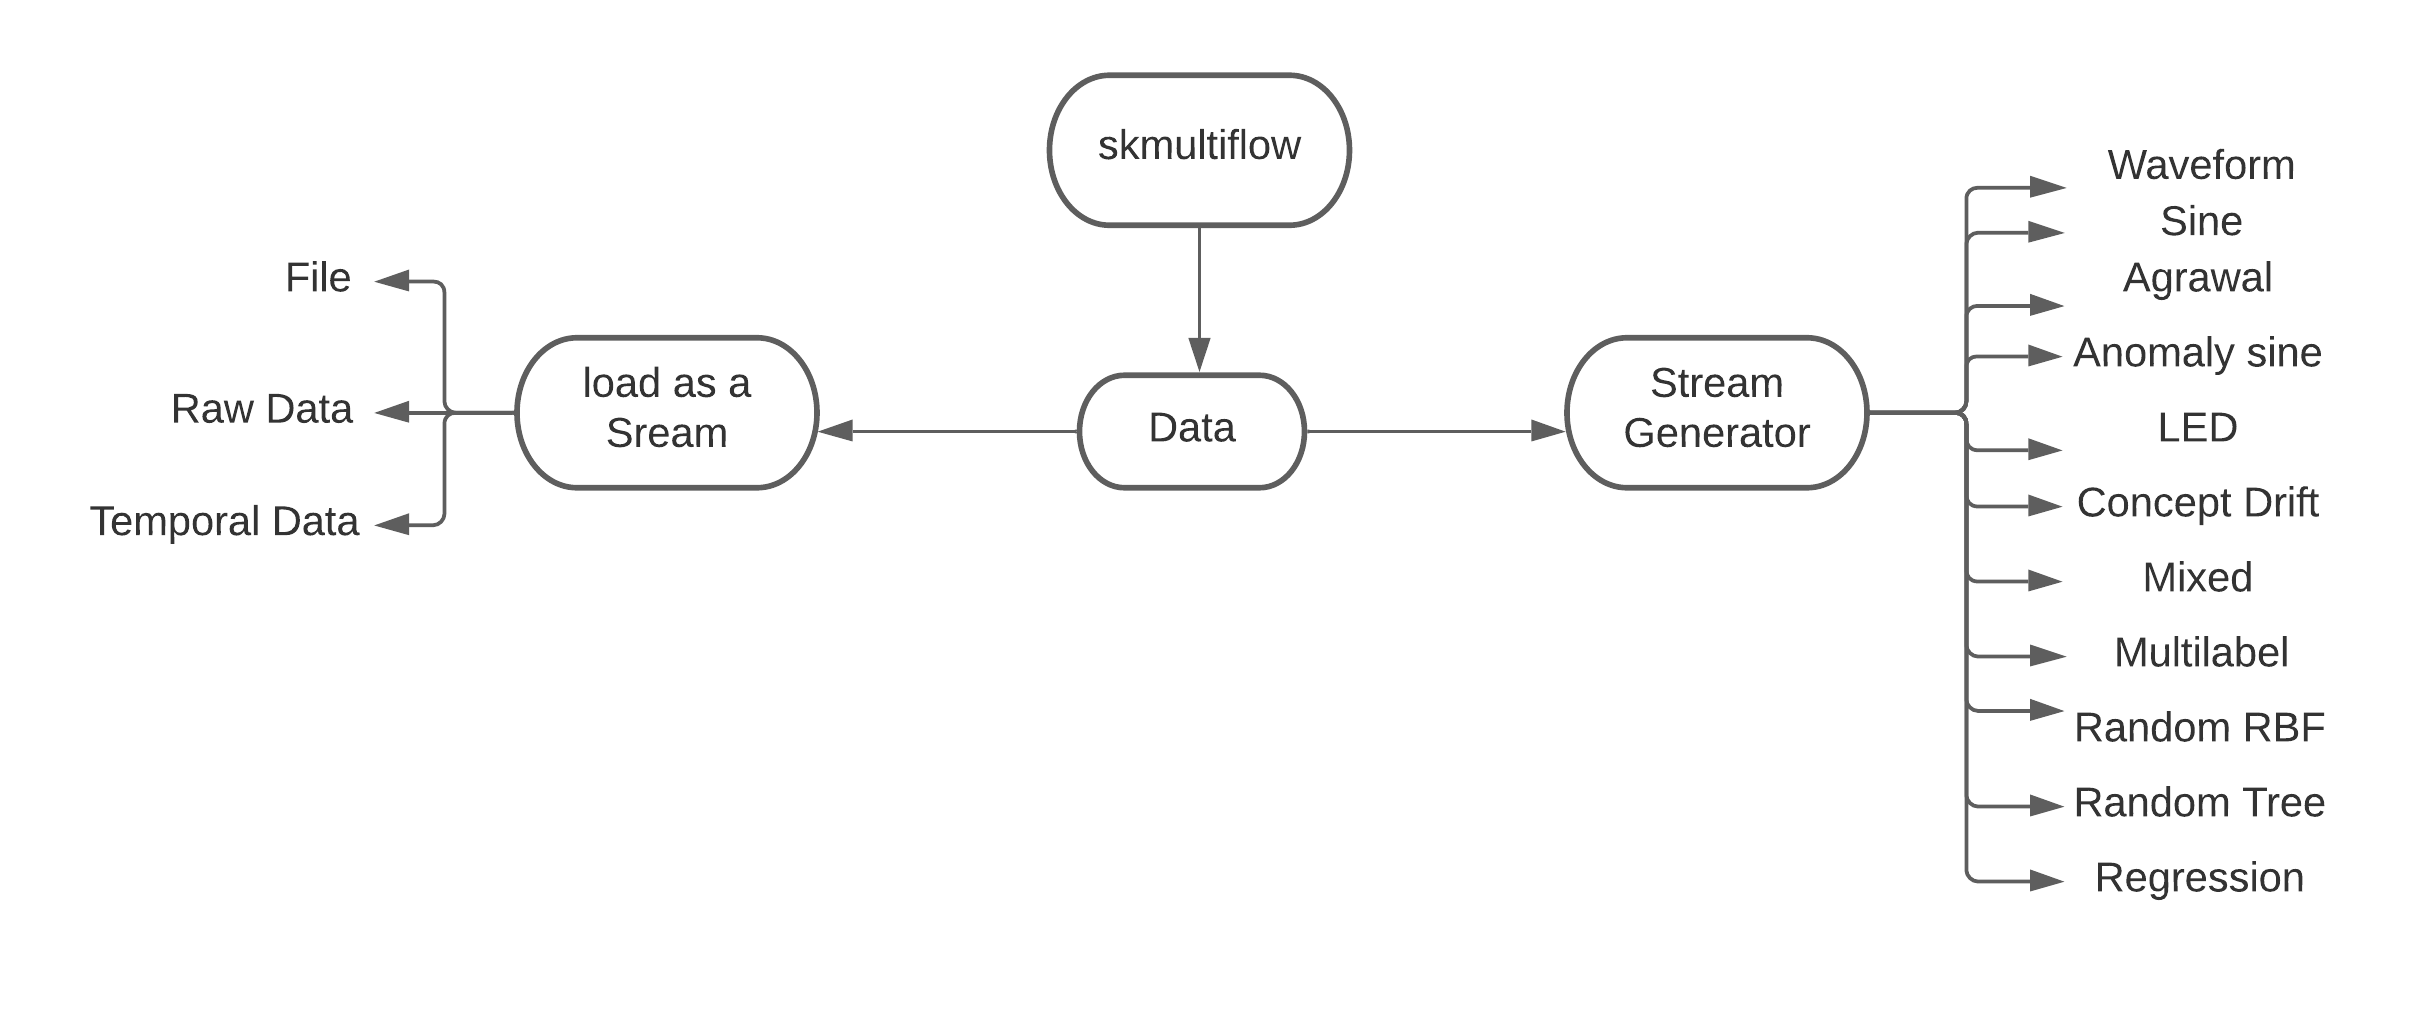
\includegraphics[width = 12cm,height = 6cm]{image/sci2.png}
% \caption{The scikit-multiflow map with multiple methods for generating data. }
% %\cite{SMF}}
% \label{sci}
% \end{figure}



% The k-means algorithm can be explained by the following 4 steps:
% Step 1: define the number of clusters (K) and randomly pick k instances as the initial cluster centroids.
% Step 2: assign all data points to the closest centroid by measuring the distance such as the Euclidean distance.

% Step 3: re-compute the centroid of each cluster by calculating mean value of all the data points in the cluster.
% Step 4: repeat steps 2 and 3 until the centroid does not change.
% https://pdfs.semanticscholar.org/1040/6a6e1319a48e731db73ed22bbde61fa42691.pdf


% \section{Comparison  Between  DSAP  and  Streaming  K-means Phase}
% The general approach of the various stream clustering algorithms that allow for the investigation of the cluster structure at different time intervals are fairly similar. They typically have two stages, online where the algorithm maintain a summary of the data as micro-clusters and next in the offline phase the summary micro-clusters are clustered to provide real insights to the data. The efficiency of these algorithms are greatly affected by the choice of the clustering algorithm used. We have introduced the DSAP algorithm for data stream clustering which is implemented based on the AP algorithm. This model is compared with the established streaming K-means algorithm introduced earlier in Chapter 2. It is known that the AP algorithm usually generates results that show that the k-means algorithm is faster than AP. However, streaming AP based algorithms has been shown to provide similar quality clusters as k-means based ones but, the results tend to be more robust.

% K-means algorithm is scalable for large datasets with different shapes and sizes and is easy to implement. The K-means algorithm is known to easily adopt to new centroids and is one of the fastest algorithms out there owing to a linear time complexity. Also, K-means guarantees convergence by trying to minimize the total sum of the square error as an objective function over the number of iterations. On the other hand, the K-means algorithm has some known drawbacks. Finding the $k$ optimum number of clusters is not a precise task that can be accurately automated. The algorithm results are a function of the initial clusters chosen and necessitate multiple runs of the algorithm with the different values to pick the most suitable clusters. During data stream clustering this process can be time consuming and make the model less accurate. The algorithm is known to have difficulties in finding the right clusters for data with varying size and density. In addition, K-means clusters centroids are affected by outliers since the mean as a statistic is sensitive to outliers. %it means outliers can drag the centroids or they may have their own centroids. 
% Lastly, even though K-means can be easily scaled to large datasets but it has difficulties to cluster high-dimension data. 


% In comparison with the K-means algorithm that needs to determine the optimal number of clusters prior by applying some methods like elbow method, the AP algorithm calculates the number of clusters internally. However, AP needs additional parameters like the damping factor and preference to be set since the model convergence is dependent on the damping parameter while the preference controls the probability of finding centroids. Due to the additional complexities in the calculation of AP it becomes prohibitively expensive to scale AP as compared to the K-means which scales linearly with the size of the dataset. The semi-supervised selection of the number of clusters in K-means limits the potential of producing large number of clusters that can sometimes be generated by the AP if it's parameters are not chosen carefully. Both these partitioning based algorithms can be evaluated based on metrics that quantify the density and spread of the clusters. 

% Affinity propagation has been shown to perform well in pattern recognition applications in the fields of computer vision and computational biology. The main advantage of AP is the robustness of its optimization. While K-means follows a greedy optimization method to find the optimum of the optimization problem, AP tackles a continues optimization problem, in which all data points are potential candidate at the beginning and clusters are gradually identified. AP does not suffer from the initialization can guarantee global optimization consistently.


